\chapter{Revisão bibliográfica\label{cap: revisao}}

Aqui são apresentados conceitos prévios necessários ao desenvolvimento e à compreensão do trabalho desenvolvido. São abordados os seguintes tópicos:

\begin{itemize}
 \item Nomenclatura básica para o estudo da dinâmica de vagões ferroviários
 \item Configuração dos vagões ferroviários de carga
 \item Dinâmica multicorpos
 \item Modelos estruturais para a via permanente
\end{itemize}


%%%%%%%
\section{Uma visão geral do sistema ferroviário}

No que segue, os vagões, truques e a via férrea são descritos de maneira genérica, com o objetivo de se ter uma visão mais global. Cada um desses subsistemas serão detalhados mais à frente neste mesmo capítulo.

\subsection{O vagão ferroviário}
Independentemente da configuração particular de um vagão, seja ele para o transporte de cargas ou de passageiros, todos possuem alguns elementos comuns. O espaço destinado à acomodação do objeto de transporte do veículo normalmente é chamado de \textit{caixa}. As caixas são conectadas ao trilhos por conjuntos mecânicos conhecidos como \textit{truques} (na literatura internacional em inglês, os truques recebem os nomes de \textit{truck} ou \textit{bogie}, sendo o último termo mais utilizado no caso de passageiros). Os truques são, do ponto de vista dinâmico, a estrutura que mais diferencia os diversos tipos de vagão, pois é neles que são montados sistemas de suspensão, esterçamento, frenagem e monitoramento específicos para o tipo de objeto a ser transportada. \citeonline{orlova_anatomy_2006} mostram um compêndio bastante extenso sobre as diversas opções para a construção mecânica de truques tanto para cargas quanto para passageiros.

O contato dos truques com os trilhos é dado por meio de rodas de aço forjado ou, em alguns casos, fundido. As rodas modernas possuem um formato cônico com a parte de maior diâmetro voltada para o lado interno do vagão. Esse perfil provou-se mais interessante do que o de rodas cilíndricas, pois auxilia na centralização do veículo em relação à e reduz a probabilidade de contato com as flanges \cite{shabana_computer_1998}, que são regiões da roda não pertencentes ao cone de contato. Em geral duas rodas do veículo são ligadas por um eixo rígido, formando o que é conhecido como rodeiro (\textit{wheelset} em inglês). Os rodeiros são de importância fundamental para a dinâmica da composição ferroviária, a ponto de \citeonline{wickens_fundamentals_2003} considerá-los como ``a unidade básica de um veículo ferroviário'' (tradução do autor). A Fig.~\ref{fig: rodeiros ferroviários} mostra rodeiros ferroviários desmontados de seus truques para inspeção de manutenção.zotero

\begin{figure}
    \centering
    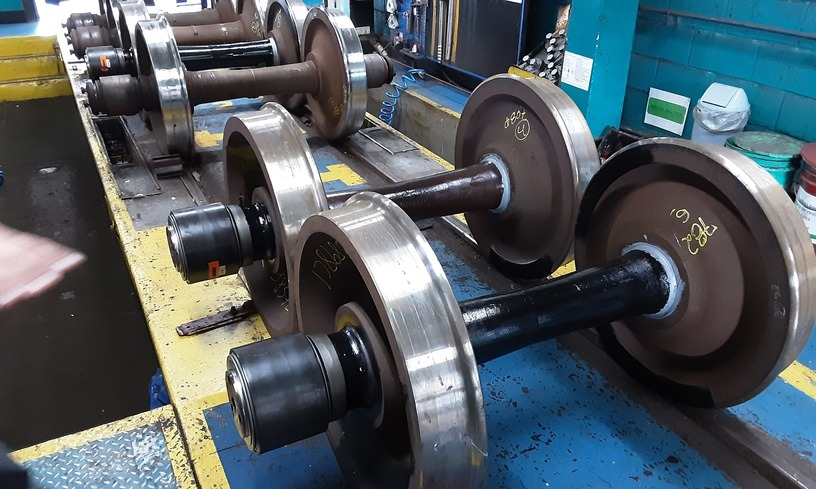
\includegraphics[width=0.6\textwidth]{Cap_2/Figuras/foto_rodeiros_vale.jpg}
    \caption{Rodeiros ferroviários alinhados para inspeção na oficina de vagões da Estrada de Ferro Vitória a Minas. Foto do autor.}
    \label{fig: rodeiros ferroviários}
\end{figure}

Em veículos de carga\footnote{Na prática ferroviária no Brasil, é comum adotar-se o termo \textit{vagão} exclusivamente para o transporte de carga e \textit{carro} exclusivamente para
o transporte de passageiros. A partir deste ponto do texto, para seguir essa convenção, subentende-se que vagões são sempre de carga e que carros são sempre de passageiros. Isso reflete, de certa maneira, a nomenclatura inglesa de \textit{wagons} e \textit{coaches}. Cabe indicar, também, que no Brasil é comum distinguir-se entre vagões de minério (responsáveis por \SI{70}{\percent} das TKU transportadas no país) e vagões de carga geral.}, os rodeiros são conectados ao truque por meio de mancais de rolamento montados sobre \textit{adaptadores}, que em geral são considerados como a \textit{suspensão primária} do veículo . Devido à alta rigidez desses mancais, apenas frequências bastante altas são filtradas por esse sistema e cabe à \textit{suspensão secundária} absorver e dissipar a maior parte do espectro de excitações provenientes da via. Mais recentemente, especialmente em vagões de tara mais alta, passou-se a utilizar sapatas de elastômero entre o adaptador e as laterais dos truques para promover uma melhor inscrição dos rodeiros em curva (ver mais à frente, na seção~\ref{sec: tpt}).

No caso de carros de passageiro o usual são duas suspensões com características de rigidez menos díspares, que deem conta tanto de excitações provenientes da via, normalmente até \SI{50}{\hertz}, e de defeitos nas rodas, caso em que as frequências podem atingir valores superiores a \SI{100}{Hz} \cite{barbosa_aplicacao_1999,knothe_modelling_1993}.

Essa separação em duas suspensões com papéis diferentes se deve, em grande medida, aos problemas de instabilidade por \textit{hunting} descritos no Cap.~\ref{cap: intro} e abordado nos trabalhos de \citeonline{redtenbacher_gesetze_1855,carter_action_1926,matsudaira_shimmy_1952} e \citeonline{wickens_dynamics_1965}. Com a experiência acumulada na operação ferroviária e os trabalhos teóricos citados, notou-se que as vibrações auto-excitadas associados ao \textit{hunting} poderiam ser minimizadas por meio de escolhas adequadas de valores para a rigidez da suspensão secundária. Paralelamente, critérios de conforto e o aumento expressivo das velocidades médias praticadas em ferrovias levaram à adoção de suspensões primárias mais sofisticadas.

Há uma classificação padronizada, no Brasil, para identificação de vagões dada pela NBR 11691 \cite{associacao_brasileira_de_normas_tecnicas_vagao_2019}. Trata-se de um código alfanumérico composto por três grupos de informação: o grupo A, formado por três letras, identifica o tipo de vagão; o grupo B contém seis algarismos que mostram a empresa proprietária do vagão e o seu número de série; o grupo C contém apenas um algarismo de controle. Para este trabalho, é relevante apenas o grupo A que, como indicado, possui três letras no formato $X_1X_2X_3$. O código $X_3$, o último, corresponde à carga máxima do vagão (Tab.~\ref{tab: carga nominal vagao ABNT}), enquanto que as duas primeiras letras indicam o tipo do vagão (Tab.~\ref{tab: tipo vagao ABNT}). Os tipos mais predominantes na frota nacional, devido ao tipo de produto transportado e às condições de carregamento e descarregamento nos terminais portuários e multimodais, são 
os gôndola por descarregamento por virador (especialmente GDE e GDT) e os \textit{hoppers} com tremela para descarregamento inferior. Com a diversificação nos tipos de
carga transportada, houve um aumento também dos plataforma para transporte de contêineres e dos vagões tanque.

Atualmente os vagões brasileiros operam com pesos brutos entre \SI{80}{\tonne} e \SI{100}{\tonne}, o que implica em cargas estáticas por eixo que variam de \SI{20}{\kilo\newton} a \SI{32,5}{\kilo\newton}.

\subsection{O truque de três peças \label{sec: tpt}}
No Brasil, bem como nos EUA, parte do leste Europeu, Rússia, Austrália e Suécia, o truque mais empregado no transporte de cargas é o truque de três peças, um sistema cujas origens remontam ao final do séc.~XIX e que teve seu desenvolvimento histórico muito influenciado pela redução dos custos de produção. Seu nome vem dos três componentes que formam sua estrutura principal: duas laterais (\textit{sideframes}) e uma travessa (\textit{bolster}) dispostos em um formato que lembra a letra ``H'', usualmente chamado, no Brasil, de \textit{aranha} (em inglês, \textit{frame}). De fato, conforme informa \citeonline{hawthorne_recent_1996}, inicialmente o termo ``três peças'' era aplicado somente à estrutura do truque (\textit{three-piece truck frame}). O termo acabou sendo adotado como sinônimo do tipo de truque com o tempo.

\begin{figure}[]
 \centering
 \begin{tikzpicture}[
tectext/.style = {
    append after command={% <= for the border
        \pgfextra{%
            \begin{pgfinterruptpath}\begin{pgfonlayer}{foreground}
            \draw[-,line width=\pgflinewidth] let \p1=($(\tikzlastnode.south west)$),
                \p2=($(\tikzlastnode.south east)$) in
                (\p1) -- (\p2);
            \end{pgfonlayer}\end{pgfinterruptpath}
        }
    }
}]

\node[anchor=south west,inner sep=0] (image) at (0,0) {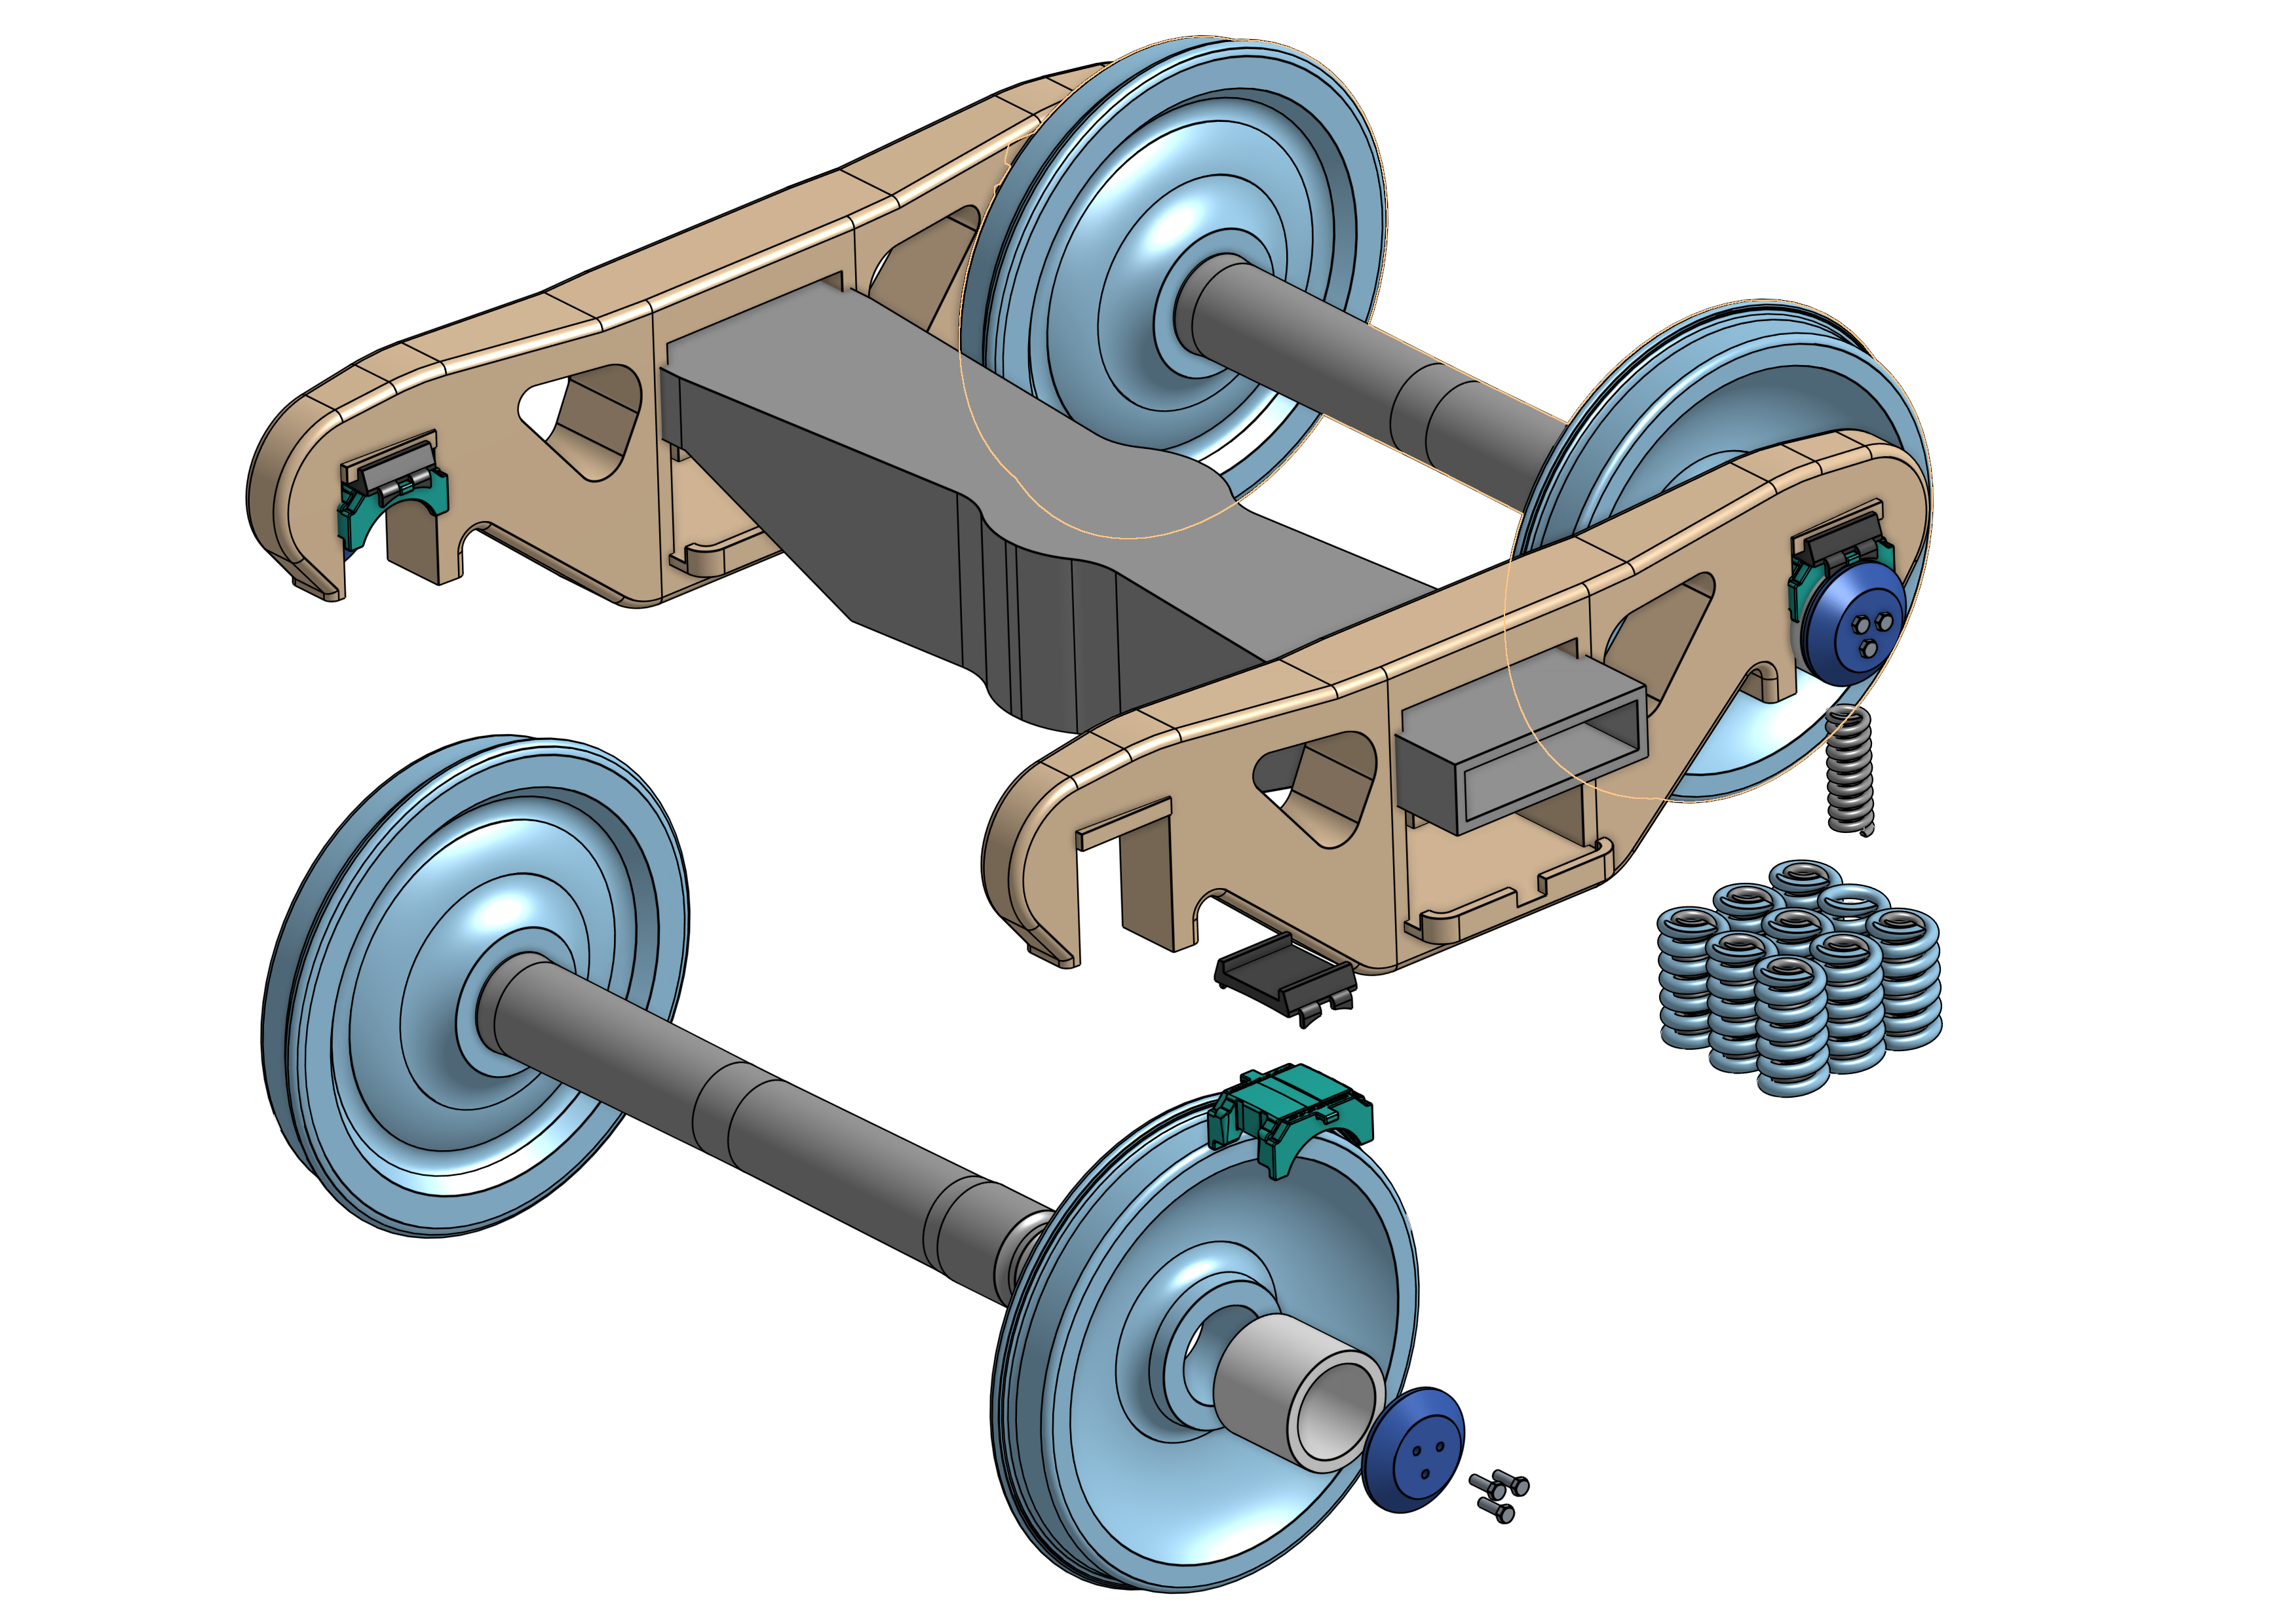
\includegraphics[width=0.6\columnwidth]{Cap_2/Figuras/truque_explodido_new.png}};
    \begin{scope}[x={(image.south east)},y={(image.north west)}]
        % \draw[help lines,step=.1] (0,0) grid (1,1);
        % \draw[help lines,step=.025,dashed] (0,0) grid (1,1);
        \draw[stealth-](0.53,0.15) -- (0.4,0.08) node[tectext,anchor=south east]{Caixa de mancal};
        \draw[stealth-](0.53,0.3) -- (0.4,0.18) node[tectext,anchor=south east,fill=white,fill opacity=0.6,text opacity=1]{Adaptador};
        \draw[stealth-](0.54,0.40) -- (0.4,0.38) node[tectext,anchor=south east,fill=white,fill opacity=0.6,text opacity=1]{Sapata};
        \draw[stealth-](0.44,0.94) -- (0.26,1.05) node[tectext,anchor=south east,]{Lateral};
        \draw[stealth-](0.49,0.49) -- (0.225,0.575) node[tectext,anchor=south east]{Pedestal}; 
        \draw[stealth-](0.48,0.70) -- (0.26,0.87) node[tectext,anchor=south east]{Travessa};
        \draw[stealth-](0.80,0.8) -- (0.95,0.87) node[tectext,anchor=south west]{Rodeiro};
        \draw[stealth-](0.81,0.38) -- (0.95,0.28) node[tectext,anchor=south west,text width=4cm]{{Molas da suspensão secundária}};
        \draw[ultra thick, rounded corners,dashed] (.50,.45) rectangle (.69,0.055) 
        node[anchor=north west,shift={(-0.08,0)},text width=1] {{Suspensão \\ {primária}}};
    \end{scope}
\end{tikzpicture}
 \caption{Truque de três peças típico (adaptado de \citeonline{lima_effect_2022})}
 \label{fig:3piece truck}
\end{figure}

A Fig.~\ref{fig:3piece truck} mostra um truque de três peças com alguns de seus principais componentes. Os rodeiros ligam-se às laterais por meio da caixa de rolamento (ou caixa de eixo, ou caixa de mancal), que contém mancais de rolamento, usualmente do tipo cartucho. Sobre o mancal há um adaptador, que é um componente de ferro fundido que compatibiliza a superfície cilíndrica do mancal com o apoio plano presente na lateral, conhecido como pedestal. Para melhorar as características de inscrição em curva dos truques, recentemente introduziu-se uma sapata elastomérica entre o adaptador e o pedestal. Esse componente reduz a rigidez de guinada do rodeiro, o que facilita seu alinhamento com o raio da curva e, consequentemente, reduz o desgaste da roda -- especialmente do friso da flange. \citeonline{lima_effect_2022} desenvolveram um método para avaliar as propriedades mecânicas da sapata a partir de medições e calibração de um modelo de elementos finitos e mostraram que a importância da rigidez vertical desse componente é pequena, mas que sua rigidez longitudinal tem grande influência no desempenho do vagão.

Entre as laterais e a travessa existe uma cama de molas helicoidais que podem variar bastante em rigidez e quantidade. Por uma questão de intercambialidade de peças, as molas são normatizadas pelas normas S-332 a S-338 da \citeauthor{association_of_american_railroads_section_2019} (AAR), que estabelecem categorias D2, D3, D4, D5, D6, D6A e D7, com rigidez e diâmetros externos crescentes. Essas molas também podem ser agrupadas em pacotes concêntricos contendo de duas a quatro molas, segundo as normas AAR de S-339 a S343. Por se tratar de componentes de dimensões não desprezíveis, o comportamento de rigidez tridimensional dessas molas é importante para a dinâmica do veículo, ou seja, do ponto de vista de modelagem física as molas devem ser consideradas como tendo rigidez em todos os seis graus de liberdade possíveis e não apenas no sentido do seu eixo \cite{baruffaldi_effects_2017}.

A dissipação da energia cinética é dada por cunhas de atrito (\textit{friction wedges} ou \textit{friction dampers}, na literatura em língua inglesa) que ficam em contato tanto com a travessa quanto com as laterais. Segundo \citeonline{hawthorne_recent_1996}, o amortecimento por atrito foi introduzido em 1935 pela Standard Car Truck Company como uma maneira de melhorar a resposta em frequência da suspensão secundária; a partir da década de 1940 já são encontrados truques com cunhas de atrito muito semelhantes às atuais. Esse tipo de componente é, do ponto de vista dinâmico, um dos itens mais interessantes no truque de três peças, já que é responsável por boa parte das não-linearidades presentes. Devido à natureza das interações de atrito, o movimento da travessa em relação às laterais está sujeito a fenômenos como adesão-deslizamento (\textit{stick-slip}), formação de ciclos limites e caos. \citeonline{kaiser_modeling_2002} mostrou com um modelo bidimensional sem perda de contato que dependendo dos parâmetros construtivos das cunhas, há o aparecimento de caos na resposta da suspensão secundária o que implica em dizer que a evolução temporal do comportamento da suspensão é muito dependente das condições iniciais. \cite{xia_modelling_2002} utilizou atrito de Coulomb bidimensional e mostrou que além de introduzir fenômenos muito não-lineares na dinâmica vertical do veículo, as cunhas também acabam por acoplar excitações laterais e verticais da travessa. A necessidade de representar com maior realismo os comportamentos não lineares da cunha levou, então, ao desenvolvimento de modelos matemáticos mais complexos do que os elementos de atrito simples utilizados até o início dos anos 2000. \citeonline{klauser_modeling_2004} apresentou um método de modelamento utilizando alguns pontos de contato virtual, mais tarde implementado no pacote padrão do programa NUCARS, que não aumenta significativamente o tempo de cálculo das simulações multicorpos. \citeonline{chandiramani_experimental_2006} montaram uma bancada em escala reduzida e constataram a presença constante de fenômenos de adesão-escorregamento, comprovando alguns dos resultados teóricos de \citeauthor{kaiser_modeling_2002}. \citeonline{steets_multibody_2007} apresentaram um modelo tridimensional que leva em consideração a distribuição dos pontos de contato entre as cunhas, as laterais e a travessa.

Sobre a travessa fica apoiada a caixa do vagão, conectada ao prato pião (\textit{bearing plate}), dispositivo que permite liberdade de guinada ao vagão. Para conter as oscilações de rolagem (rotação ao redor do eixo da via) são utilizados dois ampara-balanços por truque. Tais elementos podem ser de contato permanente, caso em que uma mola é utilizada para mantê-los sempre em contato com a caixa do vagão, ou de roletes, caso em que o vagão só entra em contato com o ampara-balanços quando tem um ângulo suficientemente alto de rolagem. O primeiro modelo tem a vantagem de garantir maior estabilidade de rolagem, mas o problema de introduzir um maior momento de resistência à guinada (o que é problemático principalmente em vias de raio de curva pequenos). O segundo modelo, por sua vez, apresenta características contrárias: menor resistência à rolagem e à guinada.

Para o leitor interessado, recomenda-se a leitura do artigo de \citeauthor{hawthorne_recent_1996} citado neste parágrafo e do texto de \citeonline{orlova_anatomy_2006}.

\subsection{Via permanente}
Dá-se o nome de \textit{via permanente} ao conjunto composto por trilhos, fixações, dormentes, lastro e subleito sobre os quais se movimenta a composição ferroviária. A Fig.~\ref{fig:comps da via permanente} apresenta um modelo simplificado para a dinâmica vertical-lateral de um vagão apoiado sobre uma via permanente típica.

\begin{figure}[]
 \centering
 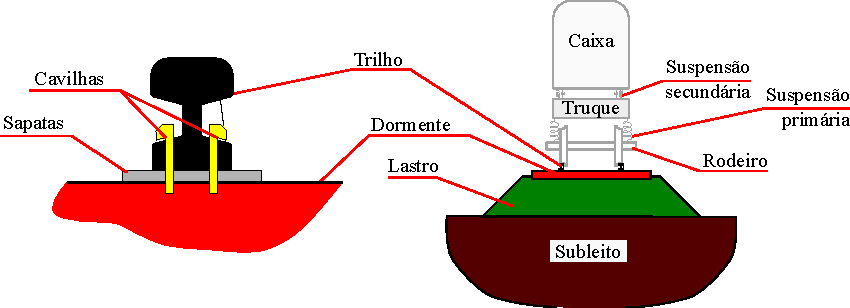
\includegraphics{Cap_2/Figuras/viaPermanente_comps.pdf}
 \caption{Modelo simplificado de vagão apresentando componentes da via permanente (adaptado de \citeonline{guimaraes_alise_1999})}
 \label{fig:comps da via permanente}
\end{figure}

A Fig.~\ref{fig: partes do trilho} mostra as três regiões principais do perfil de um trilho, que são fabricados em aço, com o boleto -- região superior, que faz contato com as rodas -- endurecido para suportar as pressões de contato envolvidas. A parte inferior dos trilhos, chamada de patim, fica conectada aos dormentes, estruturas em forma de paralelepípedo dispostas transversalmente fabricadas usualmente em madeira, aço ou concreto. É usual prender-se o trilho ao dormente por meio de cavilhas ou grampos de aço que fazem a retenção vertical, evitando o descolamento da base do trilho. Uma sapata é também utilizada com bastante frequência para aumentar o amortecimento das vibrações, principalmente quando a rigidez do dormente é mais elevada.

\begin{figure}
    \centering
    \begin{tikzpicture}[x=1in,y=1in,scale=0.3]
        \begin{scope}[rotate around={1.43:(0,0)},shift={(0,0)}]
            \draw[thick,pattern=north west lines] (0,0) -- (3-1/16,0) arc (270:360:1/16) -- (3,7/16) arc (0:75.964:1/8) -- 
            (1.042,0.927) arc (255.964:186.623:3/4) arc (186.623:180:20) arc (180:171.246:8)
            arc (171.246:139.418:3/4) arc (139.418:104.036:5/16) -- (1.233,5.682)
            arc (-75.964:1.432:5/16) -- (1.449,6.756) arc (1.432:68.597:9/16) arc (68.597:87.134:1.25) 
            arc (87.134:90:14);
            \draw[thick,xscale=-1,pattern=north west lines] (0,0) -- (3-1/16,0) arc (270:360:1/16) -- (3,7/16) arc (0:75.964:1/8) -- 
            (1.042,0.927) arc (255.964:186.623:3/4) arc (186.623:180:20) arc (180:171.246:8)
            arc (171.246:139.418:3/4) arc (139.418:104.036:5/16) -- (1.233,5.682)
            arc (-75.964:1.432:5/16) -- (1.449,6.756) node (A) {} arc (1.432:68.597:9/16) arc (68.597:87.134:1.25) 
            arc (87.134:90:14);
        \end{scope}

        \begin{scope}[rotate around={-1.43:(-10,0)},shift={(-10,0)}]
            \draw[thick,pattern=north west lines] (0,0) -- (3-1/16,0) arc (270:360:1/16) -- (3,7/16) arc (0:75.964:1/8) -- 
            (1.042,0.927) arc (255.964:186.623:3/4) arc (186.623:180:20) arc (180:171.246:8)
            arc (171.246:139.418:3/4) arc (139.418:104.036:5/16) -- (1.233,5.682)
            arc (-75.964:1.432:5/16) -- (1.449,6.756) node (B) {} arc (1.432:68.597:9/16) arc (68.597:87.134:1.25) 
            arc (87.134:90:14);
            \draw[thick,xscale=-1,pattern=north west lines] (0,0) -- (3-1/16,0) arc (270:360:1/16) -- (3,7/16) arc (0:75.964:1/8) -- 
            (1.042,0.927) arc (255.964:186.623:3/4) arc (186.623:180:20) arc (180:171.246:8)
            arc (171.246:139.418:3/4) arc (139.418:104.036:5/16) -- (1.233,5.682)
            arc (-75.964:1.432:5/16) -- (1.449,6.756) arc (1.432:68.597:9/16) arc (68.597:87.134:1.25) 
            arc (87.134:90:14);
        \end{scope}

        \draw[suporte] (A) -- +(0,1) node (A1) {};
        \draw[suporte] (B) -- +(0,1) node (B1) {};
        \draw[cota] (A1) -- (B1) node[midway, anchor=south] {Bitola};

        \draw[thick] (-10,0) +(178.57:4) -- +(-1.43:4.5) (0,0) +(1.43:4) -- (181.43:4.5) -- +(-1,0);

        \draw [decorate, decoration = {brace,mirror}] (3.2,0) --  (3.2,1.2) node[anchor=west, midway] {Patim} ;
        \draw [decorate, decoration = {brace,mirror}] (3.2,1.2) -- (3.2,5.5) node[anchor=west, midway] {Alma};
        \draw [decorate, decoration = {brace,mirror}] (3.2,5.5) -- (3.2,7.313) node[anchor=west, midway] {Boleto};
    \end{tikzpicture}
    \caption{Trilhos pefil AREMA TR68 com indicação das regões de patim, alma e boleto. A medida da bitola da via é feita nas faces internas dos boletos dos trilhos.}
    \label{fig: partes do trilho}
\end{figure}

Os dormentes são vigas feitas de madeira, concreto ou aço e presas firmemente aos trilhos, como indicado anteriormente. As configurações mais recentes, que compreendem os de concreto e os de aço, podem ser fornecidos com base constante, caso em que os patins dos dois trilhos assentam-se em um plano único, ou com base variável, e neste caso os locais de assento dos trilhos já são inclinados de 1:20 ou 1:40 dependendo da especificação da ferrovia. No caso dos dormentes de base constante, a inclinação (ângulo de \textit{cant}) dos trilhos é imposta por sapatas de fixação de dimensões adequadas. A separação dos dormentes ao longo do comprimento da via, no sentido longitudinal do deslocamento dos trens portanto, varia entre \SI{550}{\mm} a \SI{650}{\mm}, sendo essa faixa um valor de compromisso entre os custos de colocação dos dormentes e a necessidade de suporte. Mais detalhes sobre as recomendações de dimensionamento referentes aos dormentes de concreto, aço e madeira podem ser encontrados nas normas ABNT NBR~11709, NBR~11824 e NBR~7511 respectivamente.

As ferrovias operam com uma distância fixa, chamada bitola, entre faces internas dos boletos dos trilhos e a bitola determina as características geométricas de todo o material rodante utilizado. O Brasil tem a peculiaridade de ter ferrovias em três bitolas utilizadas internacionalmente: métrica (\SI{1,00}{\m}), larga (\SI{1,60}{\m}) e padrão (\SI{1,43}{\m}). Há também trechos na chamada bitola mista, que combina duas bitolas diferentes e nesse caso são usados não dois, mas três trilhos ao longo da via.

Os dormentes apoiam-se sobre o lastro, que segundo \citeonline{pereira_paulo_andre_moraes_estudo_2018} é ``uma camada formada por material granular, posicionada acima do sublastro ou subleito, com espessuras [...] geralmente variando entre \SI{250}{\mm} e \SI{350}{\mm}''. Sabe-se que essa parte da chamada infraestrutura ou subestrutura da via (infra ou sub por estar abaixo dos dormentes, que são ainda considerados parte da superestrutura da via) é muito importante no comportamento dinâmico da ferrovia, por fornecer elasticidade e amortecimento às cargas dinâmicas provenientes das passagens das rodas sobre os trilhos, além de garantir um espalhamento das tensões, preservando assim os componentes do subleito da degradação precoce. Abaixo do lastro é usual colocar-se uma camada de material de granulometria mais fina, chamada sublastro, que tem também alguma função estrutural para a via, mas cujo principal objetivo é servir como filtro entre o lastro e o leito.
%%


\subsection{Sobre sistemas de coordenadas e a descrição da via férrea}
Por ser um veículo cuja trajetória é, a princípio, prescrita pela geometria dos trilhos, são utilizados dois sistemas de coordenadas básicos na descrição da dinâmica de trens: um sistema inercial $OXYZ$ e um sistema de coordenadas locais $O^tX^tY^tZ^t$ da via (Fig.~\ref{fig:trilhos}). Os dois sistemas inicialmente coincidem no mesmo ponto $O$, mas o sistema local segue o comprimento de arco $s$ da linha média dos trilhos. Em coordenadas inerciais, o eixo $X$ é longitudinal com sentido igual à velocidade de translação do sistema; o eixo $Z$ é vertical e $Y$ é tal que $\vec{e}_Y = \vec{e}_Z \times \vec{e}_X$, com $\vec{e}_i$ ($i=X,Y,X)$ sendo o vetor unitário associado ao eixo e o operador $\times$ indicando o produto vetorial. No sistema local, o eixo $X^t$ é tangente à linha média dos trilhos e o eixo $Z^t$ resulta da rotação do sistema devido ao ângulo de superelevação (explicada mais à frente) da via, de modo que fique perpendicular à linha imaginária que une os centros dos trilhos direito e esquerdo. Cabe ressaltar que não é incomum usar eixos $Z$ e $Z^t$ que seja positivos para baixo e muitos programas comerciais de simulação adotam essa convenção. Neste trabalho, no entanto, optou-se por manter a direção positiva para cima.

\begin{figure}
 \centering
 \asyinclude{Cap_2/Figuras/via_siscoord.asy}
 \caption{Sistemas de coordenadas inercial e local}
 \label{fig:trilhos}
\end{figure}

%%%%%%
Pode-se, então, descrever a geometria da via como a combinação da trajetória da sua linha média com desvios locais dos trilhos direito e esquerdo. Como observado anteriormente, a bitola é a distância padrão entre as faces internas dos boletos dos trilhos esquerdo e direito de uma via férrea. Define-se que maneira semelhante a meia bitola $B$ como sendo exatamente metada da bitola nominal, de modo que idealmente a distância ao longo do eixo $Y^T$ da linha central da via até as faces internas dos boletos dos trilhos seria $B$. É claro que erros de assentamento e a acomodação natural da via leva a desvios da bitola nominal e a essas desvios dá-se o nome de \textit{alargamento de bitola}, sendo positivo seu valor quando a bitola real é maior do que a nominal, e negativo quando ocorre o contrário (o estreitamento da bitola, portanto).

Além da distância entre dois trilhos em um certo corte transversal da via, importa também a chamada \textit{superelevação} ou sobrelevação, mostrada na Fig.~\ref{fig: superelevacao}  que é a diferença de altura entre os dois trilhos. Essa característica da via é importante para contrabalançar a componente lateral da aceleração quando o veículo faz curva, permitindo, assim, a manutenção de velocidades maiores com segurança. Quando um veículo sai de um trecho de via reta (ou tangente, no jargão ferroviário), há uma curva espiral de transição para o trecho circular em que tanto a curvatura como a superelevação da via são aumentadas gradativamente. Quando ocorrem mudanças muito bruscas na superelevação, com gradientes mais intensos do que os esperados para um trecho espiral da via, entende-se que ocorre um defeito de geometria da via chamado de empeno ou torção\footnote{O termo \textit{torção} não é muito comum na operação ferroviária brasileira, sendo mais usual o emprego de \textit{empeno}. No entanto, na literatura em inglês e, particularmente, nas normas técnicas tanto americanas como europeias, usa-se \textit{twist}, que é mais adequadamente traduzido como torção. Além disso, o empeno da via causa uma alteração no sistema local de coordenadas da via que corresponde, em geometria diferencial, justamente à torção da tríade de Frenet.}

As oscilações verticais dos trilhos ao longo da via devido ao afundamento de elementos da infraestrutura, ou de problemas nos dormentes, são conhecidas como defeitos de \textit{nivelamento}. Se as oscilações forem laterais, dá-se o nome de defeito de \textit{alinhamento}. É importante notar que quando há defeitos de nivelamento e alinhamento nos dois trilhos e que esses defeitos estão em fase, aparecem os efeitos de alteração de bitola e de torção indicados anteriormente.

\begin{figure}
    \centering
    \begin{tikzpicture}[every node/.style={transform shape}]
        \begin{scope}[rotate=15]
            \pic[scale = 0.1] at (3,0) {trilhoTotal};
            \pic[scale = 0.1] at (-3,0) {trilhoTotal};
            \draw[suporte] (3,0) -- +(0,3) coordinate (D);
            \draw[suporte] (-3,0) -- +(0,3) coordinate (C);
            \draw[cota] (C) -- (D) node[midway, align=center, anchor=south] {Bitola de superelevação \\ $g_s$};
        \end{scope}
        \draw[thick,rotate=15,pattern=crosshatch] (-3.5,0) -- (3.5,0) -- +(-105:1.8117) -- cycle;
        \draw[suporte] (3,0.776) -- +(-8,0) coordinate (A);
        \draw[suporte] (-3,-0.776) -- +(-2,0) coordinate (B);
        \draw[cota] (A) -- (B) node[midway,anchor=east, align=right] {Superelevação\\$h_s$};
    \end{tikzpicture}
    \caption{Superelevação da via}\label{fig: superelevacao}
\end{figure}

Como já apontado, para descrever a geometria da via, é necessária, então, uma formulação matemática da sua trajetória nominal, composta pela posição espacial da linha média da via somada aos defeitos locais de alinhamento, nivelamento, torção e alteração de bitola. Seja, então, uma curva tridimensional $\vec{t}_v(s) = \left\{x_t(s),y_t(s),z_t(s)\right\}$ que descreva a linha média da via tal que essa curva é parametrizada segundo seu comprimento de arco $s$. Da teoria das curvas espaciais discutida pela geometria diferencial, a um ponto qualquer $Q$ da via, localizado na posição $s=s_Q$, pode-se associar uma tríade ortonormal composta pelos vetores tangente $\vec{e}_x^Q$, normal $\vec{e}_y^Q$ e binormal $\vec{e}_z^Q$ à curva, chamada tríade de Frenet \cite{tenenblat_introducao_2008}, definida pelo conjunto de nove equações diferenciais de Frenet-Serrat a seguir:

\begin{align}
    \begin{split}
        \frac{d\vec{e}_x^Q}{ds} &= k(s)\cdot \vec{e}_y^Q(s) \\
        \frac{d\vec{e}_y^Q}{ds} &= -k(s)\cdot \vec{e}_x^Q(s) + \tau(s)\cdot\vec{e}_z^Q \\
        \frac{d\vec{e}_z^Q}{ds} &= \tau(s)\cdot \vec{e}_y^Q(s)
    \end{split}
    \label{eq: equações de Frenet-Serrat}
\end{align}

Nas equações acima, se $k(s) > 0 $ e $\tau(s)$ forem funções diferenciáveis definidas dentro do intervalo do parâmetro comprimento de arco $s$ em que a trajetória da via é válida, então o teorema fundamental das curvas garante que a curva $t_v$ que estamos estudando é definida se conhecermos as funções $k(s)$ e $\tau(s)$, respectivamente a curvatura e a torção da curva. Adicionalmente, se para um ponto qualquer $Q\in \vec{t}_v$ conhecermos o valor do vetor tangente $d\vec{t}_v(s_Q)/ds$ e do vetor normal $d^2\vec{t}_v(s_Q)/ds^2$, então a curva $t_v$ é única.

Uma maneira de descrever a linha média da via é, portanto, medir o comprimento de arco $s$ e, para cada valor de $s$, associar o raio de curvatura $k(s)$ e a torção da via $\tau(s)$, sendo que essa última pode ser relacionada com a superelevação $h_s$ e a bitola de superelevação $g_s$:
\begin{align}
    \tau(s) = \mathrm{atan}\left({\frac{h_s(s)}{g_s(s)}}\right)
\end{align}


%%%%
\section{Dinâmica multicorpos}

A dinâmica multicorpos (DMC) é o nome associado aos métodos e técnicas de simulação computacional de sistemas mecânicos compostos de vários corpos relacionados entre si por meio de forças. Essas forças de união podem ser resultantes de restrições, como juntas e contatos, de forças de conexão, como molas e amortecedores, de esforços externos, como atuadores, e de campo, como a gravidade. Apesar de o termo ``força'' ter sido empregado, o leitor deve entendê-lo, neste contexto, como um conjunto de forças propriamente ditas e de momentos. A rigor não há diferenciação matemática entre o estudo da dinâmica multicorpos e da dinâmica clássica, derivada dos princípios fundamentais de Newton-Euler e da mecânica analítica de Lagrange e Hamilton, sendo que a principal diferença é que a DMC formula os problemas com um viés prioritariamente matricial, visando a soluções numéricas ao invés de analíticas. Isso faz com que (a) seja muito interessante o uso de programação orientada a objetos na execução da implementação computacional dos sistemas multicorpos e que (b) nem sempre seja interessante reduzir as coordenadas descritoras do movimento a um conjunto de coordenadas mínimas, especialmente no caso de sistemas com restrições unilaterais. A redução a coordenadas mínimas, que é uma característica marcante da abordagem Lagrangeana, de fato diminui o número de equações de movimento a serem resolvidas, mas também exige que um novo conjunto de coordenadas generalizadas sejam obtidas no caso do desaparecimento ou surgimento de uma restrição (como um contato ou então um deslizamento entre dois corpos).

Assim, do ponto de vista histórico, pode-se afirmar que o estudo da dinâmica multicorpos foi iniciado por Newton, em 1686, ao estabelecer os três princípios fundamentais da dinâmica de pontos materiais. Praticamente um século depois, em 1775, Euler notou que, da mesma forma que a aplicação de um conjunto de forças $\vec{F}_i$ a um sistema está relacionada com a variação da quantidade de movimento (linear) $\vec{p}$, a aplicação de momentos $\vec{M}_{i,O}$ em relação a um ponto $O$ qualquer provoca variação da quantidade de movimento angular em relação ao mesmo ponto, $\vec{L}_O$. Como aponta \citeonline{pfeiffer_mechanical_2005}, o princípio da variação de quantidade de movimento angular não pode ser derivado diretamente das proposições de Newton, consistuindo-se uma lei física independente. As equações de Newton-Euler \eqref{eq:Eq Newton-Euler} formam, então, a fundação conceitual sobre a qual se apoia o estudo de sistemas multicorpos.

\begin{align}
\begin{split}
 \frac{d\vec{p}}{dt} &= \sum_i{\vec{F}_i} \\
 \frac{d\vec{L}_O}{dt} &= \sum_i{\vec{M}_{i,O}}
\end{split}
\label{eq:Eq Newton-Euler}
\end{align}

Embora as Eqs.~\eqref{eq:Eq Newton-Euler} sejam fundamentais, elas não descrevem como um sistema que é composto de mais de um corpo se comporta. Euler abordou esse assunto e propôs o \textit{princípio do corte}, segundo o qual se pode ``cortar'' um sistema em um determinado ponto e estudar os dois sistemas resultantes de maneira independente, substituindo-se a conexão rompida por um par de forças e momentos que respeite o terceiro princípio de Newton \cite[p. 6-7]{pfeiffer_mechanical_2005}. É com esta abordagem que a maioria dos estudantes de ensino básico e de graduação aprendem a lidar com restrições entre corpos, dando origem os diagramas de corpo livre.

Existem, porém, outros enfoques. Em seu \textit{Tratado de Dinâmica}, \citeonline{dalembert_traite_1758} sugere que quando um corpo qualquer encontra uma restrição, o movimento resultante será a composição do movimento que o corpo deveria apresentar com um movimento ``perdido'', que resulta da ação da restrição. A Fig.~\ref{fig:d'Alembert} ilustra esse princípio com o exemplo de um corpo em lançamento horizontal. Caso não houvesse o anteparo indicado, a trajetória executada pelo corpo deveria continuar a ser a parábola $y = (g/2v_0)x^2$ indefinidamente. O plano horizontal, no entanto, impõe que $y\leq{h_0}$ e, assim, haverá uma parte do movimento que será perdida e transformada no movimento de restituição indicado na figura. D'Alembert compreendeu que o movimento ``perdido'' é resultado da ação das forças de reação do sistemas.

\begin{figure}[htp]
 \centering
 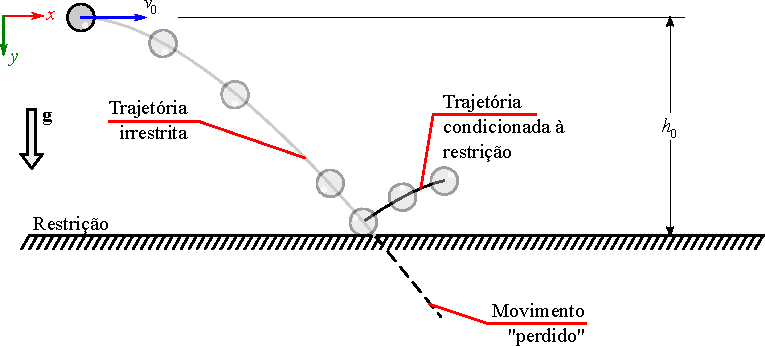
\includegraphics{Cap_2/Figuras/dalembert.pdf}
 \caption{Ilustração do princípio de d'Alembert do movimento perdido.}
 \label{fig:d'Alembert}
\end{figure}

Como aponta \citeonline{schiehlen_multibody_1997}, coube a Lagrange formular o princípio de d'Alembert em combinação com o princípio dos trabalhos virtuais. Lagrange notou que as forças que evitavam os movimentos perdidos de d'Alembert não executam trabalho. Na literatura, conhece-se como \textit{equações de movimento de Langrange do segundo tipo} \cite{schiehlen_multibody_1997,pfeiffer_mechanical_2005, woernle_mehrkorpersysteme_2011} o conjunto de equações diferenciais ordinárias derivadas a partir desse princípio. As equações de segundo tipo são escritas em função de um conjunto mínimo de coordenadas e fornecem uma maneira concisa e elegante de descrever o movimento de sistemas mecânicos. É difícil, no entanto, tratar com essas equações problemas que possuam restrições complexas, como contato intermitente ou atrito. Uma maneira de incluir esse tipo de restrição na teoria de d'Alembert-Lagrange foi apresentada em 1913 por Jourdain \cite{schiehlen_multibody_1997}, que estendeu a afirmação de Lagrange de ``as forças perdidas não realizam trabalho'' para 
``as forças perdidas não geram potência''. Com isso é possível recuperar as equações de Newton-Euler e incluir o efeito das forças de restrição por meio, por exemplo, de 
multiplicadores de Lagrange. A abordagem que a maioria dos programas de DMC usa é um misto das equações de segundo tipo de Lagrange e das equações de Newton-Euler, de modo a aproveitarem-se a formulação compacta por meio de coordenadas mínimas sempre que possível, sem perder a flexibilidade que a formulação clássica confere com relação à estrutura do sistema.

\subsection{Restrições cinemáticas\label{sec: sistemas_restritos}}
Como observado no parágrafo anterior, em alguns casos é possível encontrar um
conjunto mínimo de coordenadas que permita a descrição completa do movimento de
um sistema mecânico por meio de um sistema de equações diferenciais ordinárias.
Os elementos desse conjunto mínimo são chamados de coordenadas generalizadas
$\vec{q}$ e, de
maneira geral, são funções das coordenadas físicas do sistema $\vec{x}$, da
variação temporal (velocidades) dessas coordenadas físicas e do tempo em si:
\begin{align}
 \vec{q} &= \vec{q}(\vec{x},\dot{\vec{x}},t)
\end{align}

As coordenadas generalizadas estão relacionadas às coordenadas físicas por meio de relações de restrição. 
Suponha-se, como exemplo, uma massa de dimensões desprezíveis, solta no espaço tridimensional. Sabe-se que a posição dessa massa fica completamente definida se soubermos três parâmetros, por exemplo as coordenadas cartesianas $\{x,y,z\}$, caso em que podemos afirmar que as coordenadas físicas do problema são dadas por $\vec{x} = \{x,y,z\}$. Agora, suponhamos que essa mesma massa não esteja mais solta no espaço, mas sim presa a um ponto por meio de uma barra inextensível de comprimento $L$ que só pode se mover no plano $x-y$ e cuja extremidade sem a massa pontual está presa na origem do sistema de coordenadas. Neste caso, temos as seguinte equações de restrição:
\begin{align}
 \phi_1 &= z = 0\\
 \phi_2 &= x^2 + y^2 - L^2 = 0
\end{align}
com $L$ sendo o comprimento da barra. Dessas duas equações de restrição, vem que:
\begin{align}
 z &\equiv 0 &, \forall \{x,y\} \in \mathbb{R}^2 \\
 y &= \pm \sqrt{L^2 - x^2} &, x \leq L
\end{align}
de modo que, sabendo-se o valor da coordenada $x$, as outras duas ficam determinadas. Em outras palavras: para o sistema considerado sob a ação da restrição, um conjunto de coordenadas generalizadas é $\vec{q} = \{x\}$. O interessante é que o vetor $\vec{q}$ não é único. Mesmo para o caso simples do pêndulo descrito anteriormente, uma escolha mais interessante e igualmente intuitiva é considerar as seguintes restrições
\begin{align}
 \phi_1^* &= z = 0\\
 \phi_2^* &= r - L = 0\\
\end{align}
em que $r$ é a distância da origem à massa pontual. Nessa segunda representação, as coordenadas $\{x,y\}$ foram substituídas por $x = r\cos(\theta)$ e $y = r\sin(theta)$, com $\theta$ sendo o ângulo, assumido positivo segundo a regra da mão direita, entre o eixo horizontal e o vetor que liga a massa à origem. Nesse caso, o vetor de coordenadas generalizadas resume-se a $\vec{q}^* = \{\theta\}$

As funções $\phi_i$ utilizadas acima são chamadas \textit{restrições} do sistema e são a representação matemática de conexões, contato, ou outras condições especiais. As restrições têm o efeito de reduzir o número de possíveis movimentos do sistema e, com isso, reduzem também o número de graus de liberdade. A posição do sistema, então, pode ser compreendida como um ponto em um espaço vetorial de dimensões iguais ao número de coordenadas generalizadas e a esse espaço dá-se o nome de \textit{espaço de configurações} \cite{corben_classical_1960}. Note-se que essa compreensão das restrições como ``eliminadoras'' de graus de liberdade condiz com a noção de movimento perdido de d'Alembert.

\subsubsection{Restrições escleronômicas e reonômicas} Chamam-se \textit{restrições escleronômicas} aquelas que não são explicitamente dependentes do tempo, ao passo que às restrições que dependem do tempo dá-se o nome de \textit{reonômicas}.

\subsubsection{Restrições holonômicas e não-holonômicas} Quanto à dependência das coordenadas generalizadas (e suas derivadas), as restrições são usualmente classificadas em \textit{holonômicas} e \textit{não-holonômicas}. As primeiras tem a forma geral:
\begin{align}
 \vec{\phi}(\vec{q},t) &\leq \vec{0} \label{eq:rest holonômicas}
\end{align}
enquanto que as outras são do tipo:
\begin{align}
 \vec{\phi}(\vec{q},\dot{\vec{q}},t) &\leq \vec{0} \label{eq: rest não-holonômicas}
\end{align}

Diz-se, então, que uma restrição holonômica é dependente das coordenadas generalizadas (e do tempo, se for também reonômica) e que as restrições não-holonômicas dependem, também, das velocidades generalizadas. O tratamento de restrições não-holonômicas é, em geral, mais complicado do que o de restrições holonômicas. Felizmente, as restrições não holonômicas mais comuns dependem linearmente das velocidades generalizadas, o que pode facilitar sua manipulação. No caso do exemplo do pêndulo, as restrições $\vec{phi}_i$ são todas holonômicas escleronômicas.

\subsubsection{Restrições bilaterais e unilaterais} Existe uma última classificação, ainda, dada às restrições cinemáticas que diz respeito à sua direção de atuação ou, o que é equivalente, à direção de atuação de sua reação associada. As restrições \textit{bilaterais} são atuantes independentemente da configuração atual do sistema. A articulação entre um pistão de motor e sua biela, por exemplo, representa uma restrição do tipo $\vec{r}_{O,p} - \vec{r}_{O,b} = \vec{0}$, em que $\vec{r}_{O,p}$ e $\vec{r}_{O,b}$  representam as posições (globais) dos furos em que está posicionado o pino da articulação no pistão e na biela respectivamente. Essa restrição é bilateral, pois está ativa independentemente de o pistão estar se movendo em uma direção ou na outra. Já a restrição $y-h_0 \leq 0$ do corpo em lançamento na Fig.~\ref{fig:d'Alembert} é unilateral, pois só está ativa, isto é, ela só restringe o movimento do sistema, a partir do momento em que $y = h_0$. Em todos os instantes nos quais $y < h_0$ a restrição continua existindo do ponto de vista matemático, mas sua presença não é percebida pelo sistema e os 
graus de liberdade não são afetados por ela. Quando há restrições unilaterais em um sistema multicorpos, o número de graus de liberdade muda com o tempo, podendo aumentar ou diminuir dependendo da configuração atual. Do ponto de vista computacional isso pode ser um problema, pois o algoritmo de solução tem que adaptar a condições diferentes de restrição que podem impor não-linearidades bastante relevantes. \citeonline{pfeiffer_multibody_2004} abordam de maneira bastante completa as formulações relacionadas a problemas com restrições unilaterais.

No caso de sistemas ferroviários, as restrições unilaterais exercem um papel central, pois a interação das rodas com os trilhos é governada por uma relação desse tipo ao longo de uma topologia não linear. Além disso, devido à geometria das superfícies da roda e do trilho, é possível haver contato em mais de um ponto de contato, complicando ainda mais a análise. De maneira geral, qualquer contato intermitente deve ser considerado como uma restrição unilateral. Ainda para um veículo ferroviário de carga, existem contatos entre cunhas de atrito e componentes do truque \cite{baruffaldi_aplicacao_2010,kaiser_modeling_2002}, caixas de eixo e laterais, placa central e vagão, ampara-balanços e vagão.

\subsection{Tratamento das restrições}

Seja uma restrição bilateral holonômica (que pode ser reonômica ou escleronômica) dada por $\vec{\Phi}(\vec{x},t) = \vec{0}$. A primeira variação dessa restrição com relação às coordenadas físicas $\vec{x}$ é:
\begin{equation}
    \delta\vec{\Phi} = \frac{\partial\vec{\Phi}}{\partial\vec{x}}\delta{\vec{x}} = \vec{\Phi}_{\vec{x}} \cdot \delta\vec{x}
\end{equation}

Pela definição de restrição, qualquer deslocamento (real ou virtual) deve ser compatível com $\vec{\Phi}$, o que implica que deva ser realizado tangencialmente à hipersuperfície definida por essa restrição. Adicionalmente, é importante notar que o gradiente de $\Phi$ em relação a $\vec{z}$, $\vec{\Phi}_{\vec{x}}$ define justamente o vetor normal às restrições, de modo que se $\delta\vec{x}$ é tangente a $\vec{\Phi}$, então o produto escalar $\vec{\Phi}_{\vec{x}} \cdot \delta\vec{x}$ precisa ser nulo. Em outros termos,
\begin{equation}
    \vec{\Phi}_{\vec{x}} \perp \delta\vec{x} \label{eq: grad perp desloc}
\end{equation}

\subsection{Equações de movimento}
A dedução das equações de movimento de um sistema multicorpos mostrada a seguir baseia-se na fornecida por \citeonline{pfeiffer_mechanical_2005}. Iniciemos com a definição do  princípio de d'Alembert para um sistema composto por um único corpo $\mathcal{B}$:
\begin{align}
 \int_\mathcal{B}{\delta\vec{r}^\intercal}(\ddot{\vec{r}}dm - d\vec{F}_a) = \int_\mathcal{B}{\delta\vec{r}^\intercal w\cdot d\vec{F}_p} = 0 \label{eq:princípio de d'Alembert}
\end{align}
em que $\vec{r} = \vec{r}(x,y,z)$ é a posição de um elemento diferencial de massa no sistema de coordenadas global ou inercial, $\vec{F}_a$ são as forças ativas (que realizam trabalho) no sistema, $\vec{F}_p$ são as forças passivas (que não realizam trabalho), $\delta\vec{r}$ é a primeira variação de $\vec{r}$ respeitando as condições de restrição. O índice da integral, $\mathcal{B}$, indica que a soma é feita ao longo de todo o corpo considerado. Nota-se que o segundo termo da Eq.~\eqref{eq:princípio de d'Alembert} é análogo à relação \ref{eq: grad perp desloc}, de modo que as forças passivas devem ser, portanto, paralelas ao vetor normal da (hiper)superfície de restrições:
\begin{equation}
    d\vec{F}_p = \lambda \cdot \delta\vec{r}
\end{equation}

Derivando-se \eqref{eq:princípio de d'Alembert} duas vezes com respeito ao tempo e tomando-se a primeira variação da velocidade (respeitando-se, sempre, as restrições), chega-se ao princípio de Jourdain:
\begin{align}
 \int_\mathcal{B}{\delta^{\prime}\dot{\vec{r}}}^\intercal(\ddot{\vec{r}}dm - d\vec{F}_a -d\vec{F}_p) = 0 \label{eq:Princípio de Jourdain}
\end{align}

Para calcular a primeira variação $\delta^\prime\dot{\vec{r}}$, deve-se entender como varia a velocidade absoluta $\dot{\vec{r}}$. A posição de um ponto \textit{O} preso a um corpo qualquer $\mathcal{B}_i$ é dada por:
\begin{align}
 \vec{r}_O = \vec{r}_P + \tens{A}_i\,^{i}\vec{\rho}_{OP} \label{eq:posição ponto}
\end{align}
\begin{tabular}{ll}
 $\vec{r}_P$ & posição do ponto de referência $P$ escrito no sistema global \\
 $^i\vec{\rho}_{OP}$ & posição do ponto $O$ em relação a $P$ escrito em um sistema de coordenadas móvel fixo ao corpo \\
 $\tens{A}_i$ & tensor de rotação que transforma vetores do sistema local de $\mathcal{B}_i$ para o sistema global\\
 &
\end{tabular}

Derivando \eqref{eq:posição ponto} em relação ao tempo duas vezes, chega-se a:
\begin{align}
 \dot{\vec{r}}_O &= \dot{\vec{r}}_P + \dot{\tens{A}}_i\,^{i}\vec{\rho}_{OP} + \tens{A}_i\,^{i}\dot{\vec{\rho}}_{OP} 
 \label{eq:velocidade ponto} \\
 \ddot{\vec{r}}_O &= \ddot{\vec{r}}_P + \ddot{\tens{A}}_i{\tens{A}_i}^\intercal\vec{\rho}_{OP} + 2\dot{\tens{A}}_i{\tens{A}_i}^\intercal\dot{\vec{\rho}}_{OP} + \ddot{\vec{\rho}}_{OP} \label{eq:aceleração ponto}
\end{align}

Assume-se, por ora, que o corpo seja rígido, o que implica em afirmar $^i\dot{\vec{\rho}}_{OP} = \vec{0}$. Além disso, faz-se uso das seguintes propriedades dos tensores de rotação:
\begin{align}
 \tens{A}\tens{A}^\intercal &= \tens{E} \\
 \dot{\tens{A}}\tens{A}^\intercal &= -\tens{A}\dot{\tens{A}^\intercal} = \tilde{\vec{\omega}} \\
 \ddot{\tens{A}}\tens{A}^\intercal &= \dot{\tilde{\vec{\omega}}} + \tilde{\vec{\omega}}\tilde{\vec{\omega}}
\end{align}
com $\tens{E}$ sendo o tensor identidade e $\tilde{\vec{\omega}}$, uma matriz antissimétrica. É uma característica de matrizes antissimétricas possuírem um vetor axial associado e, no caso de $\tilde{\vec{\omega}}$, esse vetor é a velocidade angular do sistema de coordenadas cujo tensor de rotação é $\tens{A}$, escrito no sistema de coordenadas em relação ao qual o referencial se move.

Reformulando, então, a Eq. \eqref{eq:velocidade ponto}, chega-se à relação cinemática fundamental do corpo rígido e à primeira variação da velocidade \footnote{Perceba-se que na relação fundamental foi utilizada uma generalização do conceito de matriz antissimétrica associada, visto que vetores posição são radiais e não axiais. De maneira geral, a matriz $\tilde{\vec{v}}$ associada a um vetor qualquer $\vec{v}$ é \[ \tilde{\vec{v}} =
\begin{bmatrix}
0 & -v_3 & v_2 \\ v_3 & 0 & -v_1 \\ -v_2 & v_1 & 0 
\end{bmatrix}
\]} \cite{franca_mecanica_2004}:
\begin{align}
 \dot{\vec{r}}_O &= \dot{\vec{r}}_P + \tilde{\vec{\omega}}\vec{\rho}_{OP} = \dot{\vec{r}}_P + \tilde{\vec{\rho}}_{OP}^\intercal \vec{\omega} \label{eq:relação fundamental CR} \\
 \ddot{\vec{r}}_O &= \ddot{\vec{r}}_P + (\dot{\tilde{\vec{\omega}}} + \tilde{\vec{\omega}}\tilde{\vec{\omega}})\vec{\rho}_{OP} \\
 \delta\dot{\vec{r}}_O &= \begin{bmatrix}\tens{E} & \tilde{\vec{\rho}}_{OP}^\intercal\end{bmatrix}\begin{bmatrix} \delta\dot{\vec{r}}_P \\ \delta\vec{\omega} \end{bmatrix} \label{eq:Primeira variação da velocidade do corpo rígido}
\end{align}

Substituíndo-se \eqref{eq:Primeira variação da velocidade do corpo rígido} em \eqref{eq:Princípio de Jourdain}, chega-se a:
\begin{align}
 \begin{bmatrix} \delta\dot{\vec{r}}_P^\intercal & \delta\vec{\omega}^\intercal \end{bmatrix}^\intercal \int_\mathcal{B}{\begin{bmatrix}\tens{E} \\ \tilde{\vec{\rho}}_{OP} \end{bmatrix} \left\{ \left[ \ddot{\vec{r}}_P + (\dot{\tilde{\vec{\omega}}} + \tilde{\vec{\omega}}\tilde{\vec{\omega}})\vec{\rho}_{OP} \right]dm - d\vec{F}_a - d\vec{F}_p \right\}} = 0 \label{eq:Equação Jourdain movimento}
\end{align}

As definições de centro de massa $\vec{\rho}_S$ e tensor de inércia $\tens{I}_P$ são dadas por:
\begin{align}
 \vec{\rho}_S &= \frac{\int_\mathcal{B}{\vec{\rho}_{OP}}\,dm}{\int_\mathcal{B}{dm}} = \frac{\int_\mathcal{B}{\vec{\rho}_{OP}}\,dm}{m} \\
 \tens{I}_P &= \int_\mathcal{B}{\tilde{\vec{\rho}}_{OP}\,\tilde{\vec{\rho}}_{OP}\,dm}
\end{align}

Resolvendo-se, então, as integrais na Eq. \eqref{eq:Equação Jourdain movimento} chega-se à seguinte relação
\begin{align}
 \begin{bmatrix} \delta\dot{\vec{r}}_P^\intercal & \delta\vec{\omega}^\intercal \end{bmatrix}^\intercal \left\{\begin{bmatrix}m\tens{E} & m\tilde{\vec{\rho}}_S^\intercal\\ m\tilde{\vec{\rho}}_S^\intercal & \tens{I}_P \end{bmatrix}\begin{pmatrix} \ddot{\vec{r}}_P \\ \dot{\vec{\omega}} \end{pmatrix} + \begin{pmatrix} m\tilde{\vec{\omega}}\tilde{\vec{\omega}}\vec{\rho}_S \\ \tilde{\vec{\omega}}\tens{I}_P\vec{\omega} \end{pmatrix} - \begin{pmatrix} \vec{F}_a \\ \vec{M}_a\end{pmatrix} - \begin{pmatrix} \vec{F}_p \\ \vec{M}_p\end{pmatrix}\right\} = \vec{0}
\end{align}
ou, fazendo $\begin{pmatrix} \ddot{\vec{r}}_P \\ \dot{\vec{\omega}} \end{pmatrix} = \ddot{\vec{x}}$ o vetor de acelerações das coordenadas físicas, a equação pode ser reescrita como
\begin{align}
 \delta\dot{\vec{x}}^\intercal \left\{\begin{bmatrix}m\tens{E} & m\tilde{\vec{\rho}}_S^\intercal\\ m\tilde{\vec{\rho}}_S^\intercal & \tens{I}_P \end{bmatrix}\ddot{\vec{x}} + \begin{pmatrix} m\tilde{\vec{\omega}}\tilde{\vec{\omega}}\vec{\rho}_S \\ \tilde{\vec{\omega}}\tens{I}_P\vec{\omega} \end{pmatrix} - \begin{pmatrix} \vec{F}_a \\ \vec{M}_a\end{pmatrix} - \begin{pmatrix} \vec{F}_p \\ \vec{M}_p\end{pmatrix}\right\} = \vec{0} \label{eq:Eq mov Jourdain final}
\end{align}

Supondo que as restrições sejam bilaterais, tem-se que a Eq.~\eqref{eq:Eq mov Jourdain final} está sujeita às condições:
\begin{align}
 \vec{\phi}(\vec{x},t) = \vec{0}
\end{align}
cuja primeira derivada com relação ao tempo é
\begin{align}
 \dot{\vec{\phi}}(\vec{x},t) = \frac{\partial\vec{\phi}}{\partial\vec{x}}\dot{\vec{x}} + \frac{\partial\vec{\phi}}{\partial{t}} = \vec{\phi}_{\vec{x}}\dot{\vec{x}} + \frac{\partial{\vec{\phi}}}{\partial{t}} = \vec{0} \label{eq:primeira derivada das restrições}
\end{align}
Tomando-se, agora, a primeira variação na velocidade:
\begin{align}
 \delta\dot{\vec{\phi}} = \vec{\phi}_{\vec{x}} \delta\dot{\vec{x}} = \vec{0} \label{eq:ortogonalidade de velocidades}
\end{align}
A matriz $\vec{\phi}_{\vec{x}}$ é conhecida como o Jacobiano das restrições.

A Eq.~\eqref{eq:ortogonalidade de velocidades} mostra que as velocidades permissíveis são perpendiculares ao Jacobiano $\vec{\phi}_{\vec{x}}$. Do estudo de geometria diferencial, sabe-se que o Jacobiano indica as direções normais a uma superfície e, portanto, a relação anterior revela, em última análise, que toda velocidade permissível é perpendicular às superfícies de restrição, reforçando o resultado da relação \ref{eq: grad perp desloc}.

Os princípios de d'Alembert e Jourdain dizem que as forças passivas não geram trabalho e nem potência, o que implica em:
\begin{align}
 \delta\dot{\vec{x}}^\intercal\,\begin{pmatrix}
                      \vec{F}_p \\ \vec{M}_p
                     \end{pmatrix} =
                     \vec{0} \label{eq:ortogonalidade de forças}
\end{align}

Comparando \eqref{eq:ortogonalidade de velocidades} e \eqref{eq:ortogonalidade de forças}, nota-se que as forças de restrição (passivas) estão contidas dentro do espaço vetorial gerado pelo Jacobiano, ou:
\begin{align}
 \begin{pmatrix}
 \vec{F}_p \\ \vec{M}_p
 \end{pmatrix} = \vec{\phi}_{\vec{x}}^\intercal\,\vec{\lambda}
 \label{eq:relação força mult Lagrange}
\end{align}
em que $\vec{\lambda}$ é um vetor de fatores de proporcionalidade conhecidos como \textit{multiplicadores de Lagrange}.

Para chegar-se à forma clássica de representação de um sistema multicorpos pelas equações de Lagrange de primeiro tipo, deriva-se novamente a Eq.~\eqref{eq:primeira derivada das restrições} com relação ao tempo:
\begin{align}
 \frac{d^2}{dt^2}\vec{\phi}(\vec{x},t) &=
		\frac{d}{dt}\left[ \vec{\phi}_{\vec{x}}\dot{\vec{x}} + \frac{\partial{\vec{\phi}}}{\partial{t}}\right] = \\
		&=
		\frac{\partial}{\partial{\vec{x}}} \left[ \vec{\phi}_{\vec{x}}\dot{\vec{x}} + \frac{\partial{\vec{\phi}}}{\partial{t}}\right] \dot{\vec{x}} + 
		\frac{\partial}{\partial{t}} \left[ \vec{\phi}_{\vec{x}}\dot{\vec{x}} + \frac{\partial{\vec{\phi}}}{\partial{t}}\right] =\\
		&=
		\vec{\phi}_{\vec{x}}\ddot{\vec{x}} + \left[ 2\frac{\partial^2{\vec{\phi}}}{\partial{\vec{x}}\partial{t}} + \frac{\partial}{\partial{\vec{x}}}\left( \vec{\phi}_{\vec{x}} \dot{\vec{x}} \right) \right] \dot{\vec{x}} + \frac{\partial^2{\vec{\phi}}}{\partial{t}^2} = \\
		&=\vec{\phi}_{\vec{x}}\ddot{\vec{x}} + \vec{w}(\vec{x},\dot{\vec{x}},t) \label{eq:segunda derivada das restrições}
\end{align}

Note-se que a Eq.~\eqref{eq:segunda derivada das restrições} establece uma relação linear com as acelerações. Com isso, é possível escrever o sistema de equações aumentado:
\begin{align}
 \begin{bmatrix}
  \tens{M} & -{\vec{\phi}_{\vec{x}}}^{\intercal} \\
  \vec{\phi}_{\vec{x}} & \vec{0}
 \end{bmatrix} \begin{pmatrix}
                \ddot{\vec{x}} \\ \vec{\lambda}
               \end{pmatrix} +
 \begin{bmatrix}
  \tens{E} \\ \vec{0}
 \end{bmatrix} \vec{h} -
 \begin{bmatrix}
  \tens{E} \\ \vec{0}
 \end{bmatrix} \vec{f}_{a} +
 \begin{bmatrix}
  \vec{0} \\ \tens{E}
 \end{bmatrix} \vec{w} = \vec{0} \label{eq:equações aumentadas um corpo}
\end{align}
com

\begin{tabular}{lll}
 $\tens{M} = \begin{bmatrix}m\tens{E} & m\tilde{\vec{\rho}}_S^\intercal\\ m\tilde{\vec{\rho}}_S^\intercal & \tens{I}_P \end{bmatrix}$, &
 $\vec{h} = \begin{pmatrix} m\tilde{\vec{\omega}}\tilde{\vec{\omega}}\vec{\rho}_S \\ \tilde{\vec{\omega}}\tens{I}_P\vec{\omega} \end{pmatrix}$, &
 $\vec{f}_{a} = \begin{bmatrix} \vec{F}_{a} \\ \vec{M}_{a} \end{bmatrix}$
\end{tabular}

O sistema de equações \eqref{eq:equações aumentadas um corpo} pode ser facilmente expandido para um sistema multicorpos somando-se as equações para cada um dos corpos escrevendo-se as restrições entre os membros do sistema. Suponha-se um sistema formado por $n$ corpos de dimensões finitas conectados entre si e ao meio por meio de $m$ equações de restrição. O sistema de equações, então, que representa o movimento deste sistema é formado por $(6n+m)$ igualdades, das quais $6n$ são relacionadas à dinâmica das coordenadas físicas $\vec{x}$  e $m$ são relacionadas às condições de contorno.


\subsection{Solução computacional das equações de movimento}
Partindo das Eq.~\eqref{eq:equações aumentadas um corpo} generalizadas para um sistema multicorpos, algumas técnicas podem ser utilizadas para resolver o sistema. Em certas situações, em especial quando as restrições do sistema são bilaterais e holonômicas, é fácil utilizar um procedimento de substituição \cite{geradin_flexible_2001,pfeiffer_mechanical_2005,shabana_multi-body_2008} para eliminar algumas das coordenadas físicas do sistema. Seja um sistema mecânico, então, composto por um total de $n$ coordenadas físicas sujeito a $m<=n$ restrições holonômicas bilaterais. Diz-se que o sistema está descrito em um conjunto de \textit{coordenadas mínimas} se for possível encontrar um vetor de coordenadas generalizadas $\vec{q} = f(x_1,x_2,\ldots,x_n,t)$ de dimensões $l = m-n$. Se for possível descrever um sistema em coordenadas mínimas, então o movimento desse sistema é governado por $l$ equações diferenciais ordinárias e pode ser resolvido utilizando-se algorítmos adequados para a solução desse tipo de ente matemático \cite{pfeiffer_mechanical_2005,pfeiffer_multibody_2004,geradin_flexible_2001,woernle_mehrkorpersysteme_2011}.

Normalmente, porém, nem todas as variáveis excedentes podem ser eliminadas ou substituídas e não é possível encontrar uma representação em coordenadas mínimas. Neste caso, as equações diferenciais de movimento (em termos de coordenadas generalizadas ou físicas) estão sujeitas a um sistema de (in)equações algébricas que são as restrições. Matematicamente, a esse conjunto de EDOs e relações algébricas que devem ser resolvidos simultaneamente dá-se o nome de sistema de \textit{equações diferenciais-algébricas}, ou EDAs. Resolver um sistema de EDAs é consideravelmente mais complicado do que resolver apenas as equações de movimento na forma diferencial pois é necessário garantir que a solução não viole (ou viole minimamente) as equações de restrição. A solução desse tipo de sistema, então, envolve um processo iterativo de incrementação da variável livre (usualmente, em mecânica, o tempo), cálculo das relações diferenciais e correção das trajetórias inicialmente estimadas.

O sistema apresentado na Eq.~\eqref{eq:equações aumentadas um corpo} garante que as trajetórias de solução das acelerações sejam condizentes com as restrições. Não são impostos, porém, limites sobre como velocidades e posições devem se comportar. Como os algoritmos de solução numérica, em geral, são elaborados sobre simplificações de primeira ou segunda ordem, erros de aproximação e arredondamento se somam e fazem com que a trajetória calculada divirja da efetiva, levando ao rompimento das restrições nos níveis de posição e velocidade. Esse é um fenômeno conhecido como espalhamento de restrições (\textit{constraint numerical drift}). As equações que, como \eqref{eq:equações aumentadas um corpo}, são restritas na aceleração são consideradas EDAs de índice três\footnote{O conceito de índice de um sistema de equações diferenciais-algébricas ainda é um ponto de pesquisa na comunidade matemática, mas a definição mais comum diz respeito a quantas vezes a variável dependente do tempo precisa ser derivada para 
chegar-se às equações algébricas. No caso de um sistema mecânico, se as restrições fossem escritas em função direta das posições $\vec{x}$, as EDAs seriam de índice um; caso fossem escritas em função de $\dot{\vec{x}}$, seriam de índice dois.}. A formulação do problema como EDAs de índice 2 ou mesmo 1 resolve o problema do espalhamento, e trabalhos recentes têm apontado nesse sentido \cite{anitescu_formulating_1997,abe_dynamics_2004}. Em artigo também recente, \citeonline{negrut_implementation_2005} apresentam uma implementação do algortimo $\alpha$ de Hilber-Hughes-Taylor (HHT-$\alpha$) para a solução estabilizada de sistemas multicorpos com EDAs de índice três. Esse método é uma modificação com amortecimento numérico aprimorado do método de Newmark, utilizado para dinâmica estrutural e apresentado, por exemplo, em \citeonline{guimaraes_alise_1999}. A formulação HHT-$\alpha$ já se econtra disponível nas versões mais modernas do programa ADAMS, um dos mais populares \textit{software} comerciais para sistemas multicorpos.

%%%%
\section{Modelos estruturais para os trilhos}
A dinâmica dos sistemas ferroviários é de interesse de duas grandes áreas da engenharia: a Civil está mais interessada nas distribuições de tensão no interior das fundações e como essas tensões variam no tempo, levando a formação e propagação de trincas e, eventualmente, à falha; a Mecânica volta sua atenção a como as vibrações transmitidas da via para os rodeiros chegam ao vagão e a como isso afeta tanto as estruturas de suporte do material rodante como a carga. O fato é que, apesar de haver essa divisão bastante clara sobre as funções de cada componente (via e veículo) no transporte ferroviário, a dinâmica dos dois sistema é fortemente acoplada, ainda mais porque as frequências naturais de via permanente de veículo ferroviário se sobrepõem em diversas faixas.

Um resumo dos diferentes tipos de possíveis modelos para a via permanente pode ser encontrado na tese de \citeonline[Cap.~3]{guimaraes_alise_1999} e no artigo de revisão publicado por \citeonline{popp_vehicle-track_1999}. A classificação de todos os modelos em famílias é complicada, visto que cada modelo bem sucedido atende necessidades diferentes e possui abordagens bastante específicas. Uma forma de categorizá-los é dividindo-os em contínuos ou discretos.

Os modelos contínuos são normalmente derivados da formulação de Timoshenko da viga de Euler-Bernoulli sobre uma fundação de Wrinkler. A maioria desses modelos supõem viga e fundação de dimensões infinitas, de modo que as condições de contorno não são relevantes para o comportamento local. A idéia de se utilizar uma viga infinita sobre fundação elástica é creditada a \citeonline{timoshenko_method_1926,timoshenko_strength_1940}, que desenvolveu soluções aproximadas para o problema a partir de funções tentativas para a deformação da viga e mostrou, ainda, a possibilidade de utilizar-se o modelo de viga infinita para investigar estruturas finitas com o auxílio do princípio da superposição \cite{hetenyi_beams_1946}. Soluções de forma fechada para a viga de Euler-Bernoulli sobre fundação elástica foram obtidas por meio da expansão da solução das equações diferenciais da viga em séries de Fourier \cite{mathews_vibrations_1958}. \citeonline{bogacz_generalization_1989} utilizaram, ao invés de uma viga de Euler-Bernoulli, uma viga de Timoshenko em suas análises e 
mostraram que os efeitos relativos ao cisalhamento podem ser importantes na propagação das ondas dependendo da velocidade de deslocamento longitudinal e da frequência de oscilação da força aplicada. Do ponto de vista de implementação computacional moderna desses elementos, o método mais usado é o dos elementos finitos interpolados por polinômios tradicionais \cite{soriano_metodo_2003,felippa_introduction_2004} ou com funções de forma aprimoradas \cite{limkatanyu_nonlinear_2013}.

Os modelos discretos são fenomenologicamente mais corretos, pois consideram o apoio individualizado fornecido pelos dormentes. \citeonline{guimaraes_alise_1999} aponta que a forma mais adequada de modelar o sistema seria considerar os dormentes como massas suspensas concentradas, ligadas aos trilhos por uma certa rigidez e conectadas a uma fundação (lastro) continuo, com perda de contato, algo que seria possível, por exemplo, com o uso do método dos elementos de contorno \cite{sapountzakis_nonlinear_2010}.

Modelos mais complexos, como o de \citeonline{wu_double_1999} levam em consideração os efeitos da distorção da seção transversal do trilho que pode ocorrer em alta frequência e qual a influência dessas distorções na interação com outros componentes da via, como os dormentes e o lastro. Esses últimos modelos, no entanto, são mais adequados para simular excitações de altíssima frequência, que normalmente só estão presentes em vias de alta velocidade.

Há cerca de duas décadas, a comunidade interessada na análise dinâmica de veículos e vias férreas tem se voltado para a integração dos modelos multicorpos com trilhos modelados como corpos flexívies \cite{schiehlen_computational_2006}. \citeonline{escalona_modelling_2013} fizeram um levantamento bastante abrangente dos avanços mais recentes. 

Um dos problemas de integrar o método dos elementos finitos à dinâmica multicorpos está no campo de deslocamentos dos elementos. Mesmo que as deformações sejam pequenas, o movimento dos corpos no espaço faz com que o deslocamento dos nós não possa ser aproximado, no caso mais geral, por funções lineares. Como observado nas seções anteriores, utilizar um sistema de coordenadas móvel para descrever o movimento dos rodeiros é interessante na dinâmica dos veículos ferroviários. Em um sistema local, muitas vezes os deslocamentos dos trilhos são pequenos o suficiente para respeitarem algumas hipóteses de linearidade de modo que seria, a princípio, possível utilizar a teoria básica de elementos finitos estruturais. Como aponta \citeonline{shabana_computer_1998}, se por um lado o uso da formulação em um sistema de referência móvel (FFRF, sigla inglesa para \textit{floating frame of reference formulation}) para incluir elementos flexíveis em um ambiente multicorpos é interessante, pois torna mais intuitiva a adição de juntas, 
forças e condições de contorno, além de permitir uma matriz de rigidez com menos não-linearidades, por outro essa formulação faz com que a matriz de massa não seja mais invariante com o tempo e limita as deformações a pequenos valores. Desde meados da década de 1990, a formulação em termos de um sistema de coordenadas absoluto, ou global \cite{shabana_dynamics_2005}, tem se popularizado tanto nos estudos acadêmicos como nas implementações computacionais por apresentar as seguintes vantagens:

\begin{itemize}
 \item Deslocamentos globais são empregados, reduzindo a necessidade de transformações de sistemas de coordenadas durante o processamento;
 \item Os elementos de viga podem ser tratados como isoparamétricos, o que permite utilizar as mesmas funções de interpolação de deslocamentos para descrever a dinâmica de corpo rígido do elemento;
 \item As deformações durante um movimento de corpo rígido são nulas;
 \item As matrizes de massa são constantes (apesar de as de flexibilidade não o serem e poderem apresentar termos não-lineares)
\end{itemize}

Em dois artigos publicados em 2001, \citeauthor{shabana_three_2001} (\citeyear{shabana_three_2001,shabana_three_2001-1}) cristalizaram a formulação de elementos de viga em coordenadas globais e deram exemplos de aplicação. \citeonline{omar_two-dimensional_2001} e \citeonline{dmitrochenko_finite_2008} usaram as mesmas bases para propor alguns elementos de vigas. \citeonline{dufva_two-dimensional_2005} aplicaram uma representação geometricamente correta da deformação da viga \cite{geradin_flexible_2001} para deduzir um elemento na formulação absoluta sem o efeito de blocagem por cisalhamento. \citeonline{gerstmayr_geometrically_2008} também utilizaram uma descrição geometricamente correta para apresentar um novo tipo de elemento de viga em coordenadas nodais absolutas baseado no modelo proposto inicialmente por \citeonline{simo_dynamics_1986}. \citeonline{sugiyama_curved_2007} apresentaram a dedução de um elemento de viga curvo com o uso de um funcional de Hellinger-Reissner, de modo a evitar o fenômeno de blocagem por cisalhamento que ocorre quando se considera apenas um campo mestre (característica da formulação variacional básica de elementos finitos). \citeonline{nachbagauer_new_2011} introduziram um elemento de viga bidimensional baseado na ideia original de \citeauthor{shabana_three_2001} de utilizar uma abordagem de mecânica do continuo, mas com integração selectiva reduzida para eliminar o efeito de blocagem. Mais tarde o mesmo modelo de elemento foi expandido para o caso tridimensional \cite{nachbagauer_structural_2013}.

Mais recentemente, \citeonline{shabana_multi-body_2008,shabana_computational_2009} propuseram uma volta à FFRF para melhorar as características de continuidade das derivadas das funções de interpolação de deslocamentos. Segundo esses autores, essas derivadas são importantes para o cálculo preciso dos esforços de contato entre roda e trilho e a formulação em termos de um sistema global de coordenadas, apesar de todas suas vantagens apontadas, não permite funções de interpolação que pertençam a $\mathcal{C}^2$ ou conjuntos de continuidade superior. Essa nova abordagem tem a desvantagem, todavia, de não garantir continuidade  de deslocamentos nos nós dos elementos e, portanto, deve ser utilizada com cautela no tratamento de grandes deformações.

\subsection{Formulação de elementos finitos em coordenadas nodais absolutas}


\section{Contato roda-trilho}
O problema de contato entre roda e trilho tem sido estudado pelo menos desde o século~XIX e é de fundamental importância para a dinâmica
ferroviária. Tanto do ponto de vista do trilho, como do ponto de vista do veículo, o contato é a via de entrada de excitações que causam 
a resposta do sistema. Não à toa, em trabalhos que utilizam técnicas de cossimulação para analisar a interação entre o veículo e a via
flexível o ponto de conexão entre os códigos costuma ser a interface roda-trilho \cite{pombo_development_2019}.

O estudo do contato usualmente é dividido entre forças \textit{normais} à superfície de contato e forças \textit{tangenciais} à superfície de 
contato. Essa divisão se justifica por esses esforços terem características diferentes do ponto de vista de suas equações constitutivas.
Os esforços normais dependem da deformação local dos corpos em contato, podendo ser calculados a partir de uma condição de impenetrabilidade
associada a uma força de restituição relacionada com a aproximação entre os corpos. As forças e momentos tangenciais, que em dinâmica ferroviária normalmente
são chamados de forças e momentos de \textit{creep}, são obtidos a partir de uma série de diferentes modelos constitutivos que devem considerar a 
existência de regiões de escorregamento dentro da área de contato. Em geral, na sua forma mais simplificada, as forças tangenciais são entendidas como
um elemento de rigidez até um certo nível de saturação e, após esse nível, aplica-se um valor proporcional à força normal (modelo de Coulomb). É possível
usar uma saturação dependente da velocidade, como ocorre no modelo do cone de atrito utilizado, por exemplo, por \citeonline{anitescu_formulating_1997},
\citeonline{pfeiffer_multibody_2004}.

\subsection{Forças normais de contato}
A abordagem mais clássica para o problema de contato normal foi desenvolvida por \citeonline{hertz_ueber_1882} sob algumas hipóteses
que são basicamente as mesmas utilizadas 85 anos mais tarde nos trabalhos de \citeauthor{kalker_rolling_1967}. \citeonline[p. 52]{knothe_rail_2017}
fazem um excelente resumo dessas hipóteses, que é reproduzido a seguir:

\begin{enumerate}
    \item \textbf{Linearidade cinemática}: ângulos e deslocamentos são bastante pequenos, a ponto de poderem ser linearizados;
    \item \textbf{Linearidade e elasticidade dos materiais}: os materiais em contato exibem comportamento elástico linear, o 
    que implica em não haver a possibilidade, segundo essa hipótese, de deformações permanentes;
    \item \textbf{Hipótese do semi-espaço}: supõe-se que as dimensões da área de contato sejam muito menores do que o restante dos
    corpos e que, portanto, esse restante de corpos pode ser entendido como um semi-espaço infinito;
    \item \textbf{Suavidade das superfícies}: as superfícies em contato são perfeitamente suaves;
    \item \textbf{Separação das propriedades de contato e estruturais}: não existe relação entre as propriedades de contato
    e as propriedades estruturais dos materiais, de modo que elas podem ser tratadas independentemente umas das outras;
    \item \textbf{Hipótese de Hertz}: as superfícies podem ser tratadas como sendo de segunda ordem;
    \item \textbf{Materiais iguais}: os materiais são idênticos no que tange às propriedades de interesse. Da hipótese 2 acima, isso
    implica em dizer que as propriedades elásticas dos materiais devem ser as mesmas;
    \item \textbf{Materiais são homogêneos}: ou seja, tem propriedades constantes ao longo de seu volume;
    \item \textbf{Materiais são isotrópicos}: as propriedades são as mesmas em qualquer direção;
    \item \textbf{Baixa velocidade de deslizamento}: quando comparada à velocidade de propagação de ondas no material.
\end{enumerate}

A hipótese 10 associada à 3 implica em dizer que se pode desconsiderar as propriedades de inércia dos corpos para efeito
de cálculo das forças normais. E, de fato, lembrando que rodas e trilhos são fabricados em aço, é bastante razoável supor
que as velocidades de deslizamento são significativamente menores do que a velocidade de propagação de ondas de tensão, especialmente
para trens de carga (que dificilmente andam a mais de \SI{80}{\kilo\meter\per\hour}) e de passageiros de média velocidade (que trafegam até \SI{180}{\kilo\meter\per\hour}).

\begin{figure}
    \centering
    \begin{tikzpicture}[scale=0.4]
  \path[draw=black,dashdotted,line
    cap=butt,line join=miter,line width=0.025pt,miter limit=4.00] (-10,0.0)
    -- (10.,0.0) node[anchor=west] {$x$};



  \path[draw=black,dashdotted,line
    cap=butt,line join=miter,line width=0.021pt,miter limit=4.00] (0.0,-10)
    -- (0.0,10) node[anchor=south]{$z$};


    % SUPERFÍCIES NÃO DEFORMADAS
  \path[draw=black,dashed,fill opacity=1.000,draw
    opacity=0.933,line join=round,line width=0.15mm,miter limit=4.00]
    (8.9266,-5)arc(21.067:158.933:9.566)
    node[pos=0.43,circle,draw,fill=black,scale=0.2](A2){};
  \path[scale=-1.000,draw=black,dashed,fill opacity=1.000,draw
    opacity=0.933,line join=round,line width=0.15mm,miter limit=4.0]
    (8.9266,-5)arc(21.067:158.933:9.566)
    node[pos=0.57,circle,draw,fill=black,scale=0.2](A1){};

    \coordinate (O) at (0,0);

    \node[anchor=north] at (A1) {$A_1$};
    \node[anchor=south east] at (A2) {$A_2$};

    \draw[-stealth] (A1) -- (A1|-O) node[midway,anchor=east]{$\vec{w}_1$};;
    \draw[-stealth] (A2) -- (A2|-O) node[anchor=south west]{$\vec{w}_2$};


    % SUPERFÌCIES DEFORMADAS
  \path[draw=black,fill opacity=1.000,draw opacity=0.933,line join=round,line
    width=0.25mm] (8.9266,-5) arc(21.067:55:9.566) to[out=145, in=0] (3.3,0.0) -- (0.0,0.0);
    \path[xscale=-1,draw=black,fill opacity=1.000,draw opacity=0.933,line join=round,line
    width=0.25mm] (8.9266,-5) arc(21.067:55:9.566) to[out=145, in=0] (3.3,0.0) -- (0.0,0.0);

    \path[yscale=-1,draw=black,fill opacity=1.000,draw opacity=0.933,line join=round,line
    width=0.25mm] (8.9266,-5) arc(21.067:55:9.566) to[out=145, in=0] (3.3,0.0) -- (0.0,0.0);
    \path[scale=-1,draw=black,fill opacity=1.000,draw opacity=0.933,line join=round,line
    width=0.25mm] (8.9266,-5) arc(21.067:55:9.566) to[out=145, in=0] (3.3,0.0) -- (0.0,0.0);

  


    % RAIOS
  \path[draw=black,line join=miter,line width=0.15mm,miter
    limit=4.00,{Circle[length=2pt,sep=-1pt]}-stealth] (0.000,-8.4386) node[anchor=north east]{$M_2$} -- +(130:9.566) node[midway,fill=white]{$R_{x2}$};
  \path[draw=black,line join=miter,line width=0.15mm,{Circle[length=2pt,sep=-1pt]}-stealth] (0.0000,8.4386) node[anchor=south east]{$M_1$} -- +(-130:9.566) 
    node[midway,fill=white]{$R_{x1}$};

  % APROXIMAÇÃO
  \draw[{Circle[length=3pt,sep=-1.5pt,fill=none]}-stealth,line width=0.15mm] (0.0,-9.566) -- (0.000,-8.4386)
    node[midway,anchor=west]{$\delta_2$};
  \draw[{Circle[length=3pt,sep=-1.5pt,fill=none]}-stealth,line width=0.15mm] (0.0,9.566) -- (0.000,8.4386)
    node[midway,anchor=west]{$\delta_1$};

    % ÁREA DE CONTATO
    \draw[suporte] (-3.3,0) -- +(0,-3) coordinate (E1);
    \draw[suporte] (3.3,0) -- +(0,-3) coordinate (E2);
    \draw[cota] (E1) -- (E2) node[midway,fill=white]{$2a$};

    % LEGENDA
    \begin{scope}[shift={(5,7)}]
        \draw[dashed] (0,1) -- (2,1) node[anchor=west]{Superfície não-deformada};
        \draw[line width=0.25mm] (0,0) -- (2,0) node[anchor=west]{Superfície deformada};
    \end{scope}
\end{tikzpicture}   
    \caption{Superfícies em contato. Adaptado de \citeonline{knothe_rail_2017}.}
    \label{fig: Hertz}
\end{figure}

A Fig.~\ref{fig: Hertz}, adaptada de \citeonline{knothe_rail_2017}, mostra dois corpos, identificados como 1 e 2, em contato. Tais corpos têm suas superfícies descritas por funções de segunda ordem e suas formas não deformadas são indicadas pelas linhas tracejadas. O sistema de coordenadas $Oxz$ é adotado para descrever o contato de maneira que o ponto $O$ está no meio da zona de contato e que $z$ é normal ao plano de contato, com sentido positivo para o centro do corpo 1. O eixo $y$ aponta para dentro do plano do papel. Quando os dois corpos são pressionados um contra o outro, suas superfícies não deformadas para atingir o formado indicado pela linha sólida, causando um amassamento das superfícies e consequente aproximação ($\delta_i$) dos centros locais de curvatura, indicados por $M_1$ e $M_2$. Ao fim da aplicação da força, forma-se uma área deformada de dimensão $2a$ (e $2b$ na direção $y$). Os valores $R_{xi}$ indicam a curvatura local em relação ao plano $xz$ e existem também os raios $R_{yi}$ que denotam a curvtura no plano $yz$, mas que não estão mostrados na figura para manter a simplicidade da representação. Como supõ-se que as superfícies sejam de segunda ordem, sabe-se que há uma relação quadrática entre os raios $R_{xi}$ e $R_{yi}$. 

A análise é feita a partir de dois pontos das superfícies dos corpos, $A_1$ e $A_2$ que, após a deformação, estarão na área de contato. Inicialmente a distância entre esses dois pontos é dada por $h_0$ e ao fim da aplicação da carga eles se deslocam verticalmente das distâncias $w_1$ e $w_2$. Assim, a distância final entre esses dois pontos -- que deve ser igual a zero, uma vez que ambos se encontram na zona de contato -- é geometricamente dada por:
\begin{equation}
    0  = h_0 - \left(\delta_1+\delta_2\right) + \left(w_1-w_2\right)
\end{equation}
|
Fazendo $\delta = \delta_1+\delta_2$, lembrando da hipótese de superfícies de segunda ordem e aplicando as curvaturas equivalentes
\begin{align}
    \begin{split}
        \kappa_x^* &= \frac{1}{R_x^*} = \frac{1}{R_{x1}} + \frac{1}{R_{x2}} \\
        \kappa_y^* &= \frac{1}{R_y^*} = \frac{1}{R_{y1}} + \frac{1}{R_{y2}},
    \end{split}
    \label{eq: raios_eqv_curvatura}
\end{align}
obtém-se a seguinte relação para aproximação entre os pontos $A_1$ e $A_2$:
\begin{equation}
    w_1(x,y) - w_2(x,y) = \delta - \kappa_x^* \frac{x^2}{2} -  \kappa_y^* \frac{y^2}{2}
    \label{eq: desl geometrico contato}
\end{equation}

Conforme as hipóteses 2 e 7, os materiais são iguais e elástico-lineares com módulo de elasticidade $E$ e 
coeficiente de Poisson $\nu$. Para cada um dos corpos, o afundamento da superfície de contato para uma 
carga pontual $Q$ a uma distância $r$ do ponto de aplicação é dado pela equação \cite{singer_introduction_1992}:
\begin{equation}
    w(r) = \frac{1-\nu^2}{\pi E} \frac{P}{r}
    \label{eq: desl forca concentrada}
\end{equation}

A pressão de contato entre os dois corpos pode ser entendida como um conjunto de infinitas forças pontuais distribuídas, 
de modo que o deslocamento de cada ponto dentro da área de contato $\Upsilon$ pode ser calculado pela integral da Eq.~\eqref{eq: desl forca concentrada}:
\begin{equation}
    w(x,y) = \frac{1-\nu^2}{\pi E} \int\int_\Upsilon {\frac{p(\xi,\eta)}{\sqrt{(x-\xi)^2 + (y-\eta)^2}}d\xi d\eta}
    \label{eq: desl area contato}
\end{equation}

Substituindo-se a Eq.~\eqref{eq: desl area contato} na Eq.~\eqref{eq: desl geometrico contato} e lembrando que 
as propriedades constitutivas dos dois materiais são as mesmas, vem que:
\begin{equation}
    2\frac{1-\nu^2}{\pi E} \int\int_\Upsilon {\frac{p(\xi,\eta)}{\sqrt{(x-\xi)^2 + (y-\eta)^2}}d\xi d\eta} = \delta - \kappa_x^* \frac{x^2}{2} -  \kappa_y^* \frac{y^2}{2}
\end{equation}
que pode ser resolvida para se encontrar a distribuição de pressão de contato que é compatível com as hipóteses citadas anteriormente. Hertz fez uma analogia com a solução
do potencial eletrostático e notou que a solução de tal equação é uma distribuição elipsoidal de pressão tal que:
\begin{equation}
    p(x,y) = p_0 \sqrt{1-\frac{x^2}{a^2} - \frac{y^2}{b^2}}
    \label{eq: pressao_hertz}
\end{equation}

O contato entre roda e trilho pode ser compreendido como a interface entre dois elipsoides, com raios de curvatura diferentes nas direções lateral
e longitudinal do deslocamento do rodeiro. A seguir segue-se a formulação de \citeonline{johnson_contact_1985} com a notação usada por \citeonline{knothe_rail_2017} e indicada na Fig.~\ref{fig: hertz_roda_trilho}. Assume-se um sistema de coordenadas locais com origem no centro
da área de contato, ponto $P_C$. O eixo $\zeta$ é normal ao plano de osculação do contato, $\eta$ está no plano que contém o eixo da roda e $\xi$
é ortogonal aos dois outros eixos, de modo que $\left\{\xi,\eta,\zeta\right\}$ formam um sistema ortogonal direito. Roda e trilho, seguindo a formulação hertziana, são entendidos localmente como superfícies quadráticas sendo que $R_{\xi i}$ e $R_{\eta i}$ são, respectivamente, os raios de curvatura das superfícies nos planos $\xi\zeta$ e $\eta\zeta$, com $i=1$ sendo a roda e $i=2$ o trilho.

\begin{figure}
\centering
    \begin{tikzpicture}[x=1mm,y=-1mm,scale=0.7]
          %\begin{scope}[cm={{0.26458,0.0,0.0,0.26458,(123.922,-98.3844)}}]


          % TRILHO
    \path[draw=black,line width=0.25mm,miter limit=4.00] (10.1876,167.3489) ..
      controls (10.6411,163.8244) and (12.0714,160.4969) .. (14.3169,157.7426) ..
      controls (15.3564,156.4676) and (16.7665,155.5470) .. (18.3520,155.1082) --
      (30.0196,151.8795) .. controls (33.5845,150.8930) and (35.9876,147.5651) ..
      (35.8028,143.8709) -- (34.9040,125.9056) .. controls (34.6167,120.1643) and
      (30.9168,115.1544) .. (25.5141,113.1911) .. controls (22.2889,112.0191) and
      (18.8951,111.3777) .. (15.4647,111.2918) .. controls (9.5371,111.1434) and
      (3.6068,111.1434) .. (-2.3208,111.2915) .. controls (-8.2484,111.4397) and
      (-14.1714,111.7361) .. (-20.0842,112.1805) .. controls (-23.5060,112.4377) and
      (-26.8635,113.2478) .. (-30.0261,114.5795) .. controls (-35.3239,116.8103) and
      (-38.7690,121.9989) .. (-38.7690,127.7473) -- (-38.7690,145.7351) .. controls
      (-38.7690,149.4339) and (-36.2026,152.6376) .. (-32.5929,153.4447) --
      (-20.7785,156.0864) .. controls (-19.1731,156.4454) and (-17.7188,157.2944) ..
      (-16.6169,158.5160) .. controls (-14.2366,161.1546) and (-12.6418,164.4064) ..
      (-12.0128,167.9039);


    % RODA
    \path[draw=black,line width=0.25mm,miter limit=4.00] (60.6913,92.7771) ..
      controls (60.6913,101.2367) and (54.0575,108.2102) .. (45.6084,108.6323) --
      (-24.5062,112.1353) .. controls (-30.7689,112.4309) and (-36.8618,114.2677) ..
      (-42.2445,117.4826) .. controls (-45.4711,119.4161) and (-47.8050,122.5441) ..
      (-48.7398,126.1876) -- (-49.6400,129.5476) .. controls (-50.0558,131.0987) and
      (-50.8571,132.5195) .. (-51.9693,133.6780) .. controls (-55.2644,137.1298) and
      (-59.8285,139.0827) .. (-64.6006,139.0827) .. controls (-70.9745,138.8046) and
      (-76.5627,134.7379) .. (-78.7873,128.7583) .. controls (-81.3167,123.9858) and
      (-83.2568,118.9236) .. (-84.5650,113.6831);


        % EIXOS
    \coordinate (CP) at (-10.06,111.14);
    \path[draw=black,line cap=butt,line join=miter,line width=0.18mm,miter
      limit=4.00,stealth-] (-52.3695,113.1004) node[anchor=east]{$\eta$} -- (CP);
    \path[draw=black,line cap=butt,line join=miter,line width=0.18mm,miter
      limit=4.00,-stealth] (CP) node[anchor=north]{$P_C$} -- (-12.1023,68.7394) node[anchor=east]{$\zeta$};
    \path[draw=black,line cap=butt,line join=miter,line width=0.18mm,miter
          limit=4.00,{Circle[length=4pt,sep=-2pt]}-stealth] 
          (CP) -- +(-15:30) node[anchor=west]{$\xi$};

    % CORTE DA RODA
      \draw[rotate=1.43,dashed] (-13.1,78.6) +(14,0) arc(0:-30:14mm and 32.8mm) coordinate (D) arc (-30:-140:14mm and 32.8mm) ;
      \draw[rotate=1.43, line width=0.18mm, Rays-stealth] (-13.1,30.6) -- (D) node[midway,fill=white] {$R_{\xi 1}$};

    \path[draw=black,line cap=butt,line join=miter,line width=0.18mm,miter
      limit=4.00,stealth-Rays] (-0.9803,111.2606) -- (-0.5323,142.6009) node[midway,fill=white]{$R_{\eta 2}$} -- (3.6592,140.9944) --
      (4.2246,167.6664);


    % área de contato
    \begin{scope}[shift={(60,50)},scale=1.5]
        \draw[pattern=north west lines] (0,0) ellipse[x radius = 10, y radius = 5];
        \draw[line width = 0.18mm,-stealth] (0,0) -- (-14,0) node[anchor=east]{$\eta$};
        \draw[line width = 0.18mm,-stealth] (0,0) -- (0,-8) node[anchor=south]{$\xi$};

        \draw[suporte] (-10,0) -- +(0,8) coordinate (A1);
        \draw[suporte] (10,0) -- +(0,8) coordinate (A2);
        \draw[cota] (A1) -- (A2) node[midway, anchor=north]{$2a$};

        \draw[suporte] (0,5) -- +(13,0) coordinate (A1);
        \draw[suporte] (0,-5) -- +(13,0) coordinate (A2);
        \draw[cota] (A1) -- (A2) node[midway, anchor=west]{$2a$};
    \end{scope}


    \end{tikzpicture}
    \caption{Representação do contato entre roda e trilho, indicando os eixos locais de contato.}
    \label{fig: hertz_roda_trilho}
\end{figure}

Define-se o rádio médio equivalente de curvatura como sendo
\begin{equation}
    R_m^* = \sqrt{R_\xi^* R_\eta^*}
\end{equation}
onde $R_\xi^*$ e $R_\eta^*$ são estabelecidos segundo a Eq.~\eqref{eq: raios_eqv_curvatura}.

Para simplificar a notação, define-se também o rádio médio da área de contato como sendo:
\begin{equation}
    c = \sqrt{ab}
\end{equation}

Pode-se mostrar, a partir da Eq.~\eqref{eq: pressao_hertz}, que 
\begin{equation}
    c = F_1(g)\cdot\sqrt[3]{\frac{3}{2}\frac{\left(1-\nu^2\right)}{E} N R_m^*}
\end{equation}
com $N$ sendo a força normal aplicada no contato e $F_1(g)$ é um fator relativo à integração da pressão
de contato sobre uma área elíptica e que depende de $g = \max\left(R_\xi/R_\eta,R_\eta/R_\xi\right)$.

Para áreas de contato pouco elípticas, isto é, que se aproximam da forma de um círculo, o valor de $F_1(g)$. 
De fato, se $g\leq5$, pode-se assumir que \cite{singer_introduction_1992}
\begin{equation}
    c \approx \sqrt[3]{\frac{3}{2} \frac{\left(1-\nu^2\right)}{E}N R_m^*}
\end{equation}
que é justamente o radio da área de contato circular entre duas esferas.

Com isso, pode-se mostrar que \cite[cap. 4]{johnson_contact_1985} a aproximação dos corpos de contato é dada por:
\begin{equation}
    \delta = \sqrt[3]{\left[ \frac{3}{2} \frac{\left(1-\nu^2\right)}{E} N R_m^* \right]^2} \frac{1}{R_m^*} F_2(g)
    \label{eq: delta_Nhertz}
\end{equation}
com $F_2(g)$ também sendo resultado da solução de integrais elípticas.

A Eq.~\eqref{eq: delta_Nhertz} estabelece, então, uma relação entre a aproximação dos corpos $\delta$ e a força normal
aplicada $N$. Em tese, é possível obter uma rigidez equivalente $k_h$ linearizada ao redor de uma deflexão $\delta_0$.
Claramente, essa rigidez depende muito dos parâmetros constitutivos do material e também da geometria das superfícies
em contato. A Fig.~\ref{fig: graf_Nxdelta} mostra o gráfico de $N$ em função de $\delta$ para valores típicos para
contato entre boleto de um trilho novo com o cone de rodagem de uma roda nova. Na carga de \SI{175}{\kilo\newton},
a rigidez equivalente aproximada é de \SI{1,66}{\mega\newton\per\m}.

\begin{figure}
    \centering
    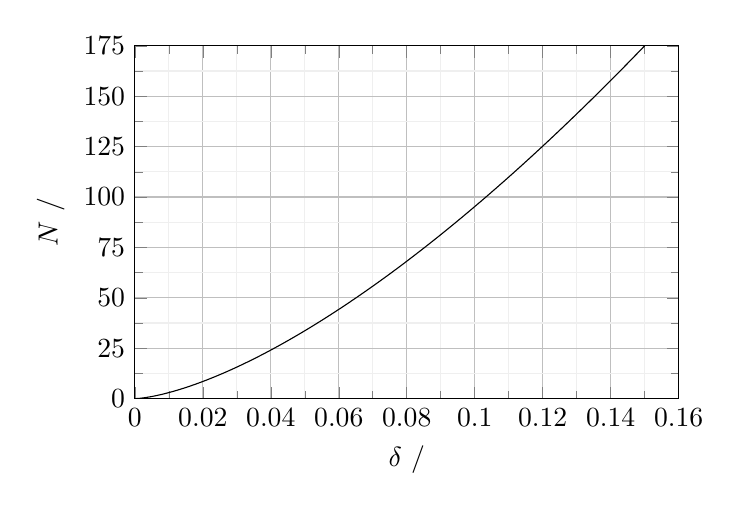
\begin{tikzpicture}
        \begin{axis}[
            xmin = 0, xmax = 0.16,
            ymin = 0, ymax = 175,
            xtick distance = 0.02,
            xticklabel style={
                  /pgf/number format/precision=2,
                  /pgf/number format/fixed},
            ytick distance = 25,
            grid = both,
            minor tick num = 1,
            major grid style = {lightgray},
            minor grid style = {lightgray!25},
            width = 0.7\textwidth,
            height = 0.5\textwidth,
            xlabel = {$\delta$ / \si{\milli\meter}},
            ylabel = {$N$ / \si{\kilo\newton}},
        ]
            \plot[domain = 0:0.16,samples=100] 
                    {3012750*x^(3/2)/1e3};
        \end{axis}
    \end{tikzpicture}
    \caption{Relação entre força e aproximação dos corpos para contato entre boleto de trilho e cone de rolamento de roda ferroviária.
    Ambos os componentes são considerados novos. Raio da roda de \SI{350}{\mm}, raio do boleto do trilho de \SI{350}{\mm},
    feitos de aço com $E=\SI{210}{\giga\pascal}$ e $\nu=\num{0,3}$.}
    \label{fig: graf_Nxdelta}
\end{figure}

Outra maneira de se encontrar uma rigidez equivalente para o contato roda trilho é utilizar a relação
proposta por \apudonline{esveld_modern_2001}{steenbergen_wheel-rail_2008}, que considera uma região de contato
circular com raio $c = \sqrt{ab}$ :
\begin{equation}
    k_h = \sqrt[3]{\frac{3}{2} \frac{E^2}{\left(1-\nu^2\right)^2}R_m^* Q_0}
\end{equation}
onde $Q_0$ é a carga estática na roda. Para os mesmos valores utilizados na estimativa do parágrafo anterior,
obtém-se uma rigidez equivalente com valor de \SI{1,70}{\mega\newton\per\m}.

É claro que para descarregamentos muito intensos da roda  em relação à carga estática,
as aproximações linearizadas acima não podem ser aplicadas e,
nesse caso, é necessário usar a Eq.~\eqref{eq: delta_Nhertz}

\subsection{Forças tangenciais}
O cálculo da força normal de contato resolve apenas parcialmente o problema da interação roda-trilho. As forças tangenciais,
de atrito, envolvem um fenômeno pode ser dividido basicamente em adesão e deslizamento. Quando ocorre adesão entre dois pontos em contato,
a velocidade relativa entre esses dois pontos é nula, ao passo que no deslizamento a velocidade relativa é finita.
No contato entre roda e trilho, numa mesma área de contato existem regiões que estão em adesão e regiões que estão em
escorregamento. O efeito macroscópico dessa combinação é que a velocidade circunferencial da roda em relação ao trilho
não é zero. 

Dentro do contexto ferroviário, faz-se uma diferenciação entre os termos em inglês \textit{creepage} e \textit{slip}, seguindo uma tradição
advinda dos estudos de \citeonline{carter_electric_1916}, que é creditado como o primeiro a reconhecer a existência
de deslizamento e adesão numa mesma área de contato \footnote{\citeonline[p.~60]{knothe_rail_2017} sugerem que Carter
tenha sido influenciado pelos trabalhos de \citeonline{reynolds_rolling_1876} sobre contato com rolamento.}. \textit{Slip},
ou \textit{escorregamento}, é a velocidade relativa de duas superfícies em uma direção tangencial ao plano de contato.
Já o \textit{creepage}\footnote{Em dinâmica de automóveis com pneus, o termo \textit{slip}
equivale ao \textit{creepage} da dinâmica ferroviária.}, que será traduzido aqui como \textit{arrastamento}, é uma grandeza adimensional 
que indica a razão 
entre o escorregamento e uma velocidade de referência.

A solução do problema tangencial de contato consiste em encontrar funções:
\begin{align}
    \begin{split}
        T_\xi &= T_\xi(\upsilon_\xi,\upsilon_\eta,\upsilon_\zeta) \\
        T_\eta &= T_\eta(\upsilon_\xi,\upsilon_\eta,\upsilon_\zeta) \\
        M_\zeta &= M_\zeta(\upsilon_\xi,\upsilon_\eta,\upsilon_\zeta) \\
    \end{split}\label{eq: creep_forces}
\end{align}
que permitam o cálculo, respectivamente, das forças de tração nas direções $\xi$ e $\eta$ e do momento de resistência
ao redor de $\zeta$ (consultar Fig.~\ref{fig: hertz_roda_trilho} para indicação das direções). Tais funções dependem 
dos arrastamentos (\textit{creepages}) $\left(\upsilon_\xi,\upsilon_\eta,\upsilon_\zeta\right)$. A solução das
Eqs.~\eqref{eq: creep_forces} é bastante complexa e existem diversas metodologias desenvolvidas por 
\citeauthor{johnson_contact_1985,kalker_fast_1982,polach_creep_2005,vollebregt_numerical_2014}, entre outros. Sem impor maiores
hipóteses, os cálculos necessários são bastante trabalhosos e, ao longo da segunda metade do séc.~XX,
notou-se que para uma parte significativa dos casos práticos, soluções simplificadas podem ser utilizadas com 
sucesso \cite{zaazaa_review_2009}. Em particular, o algoritmo chamado FASTSIM, desenvolvido por \citeonline{kalker_fast_1982},
ainda hoje é muito utilizado em simulações multicorpos nas quais o principal objetivo do contato-roda trilho
é fornecer forças de conexão entre o veículo e a via. Recentemente, o grupo de engenharia ferroviária publicou um
novo modelo que pretende substituir o FASTSIM, chamado Fastrip \cite{sh_sichani_alternative_2016}, mas que ainda
não está completamente estabelecido como alternativa.

A ideia do FASTSIM é separar a roda em $n$ fatias paralelas ao eixo $\xi$ do contato, formando algo como uma série de
troncos cônicos. Define-se que o centro de cada uma das $j$ fatias está localizado na coordenada $\eta'_j$.
As equações de contato tangencial são então resolvidas para cada fatia individualmente. Na abordagem de Kalker, 
os arrastamentos são calculados como:
\begin{align}
    \upsilon_\xi &= \frac{v_\xi - \Omega R_{\xi 1}}{V} \\
    \upsilon_\eta &= \alpha \\
    \upsilon_\zeta &\approx \frac{R_{\xi1}\sin(\gamma)}{V\gamma} 
\end{align}
onde $\gamma$ é a conicidade da roda, $V$ é a velocidade de translação da roda no sentido de $X^t$ e
$\alpha$ é o ângulo de guinada do rodeiro, ou seja, o ângulo entre o eixo de rotação do rodeiro e o eixo $Y^t$, 
projetado no plano $X^t Y^t$.

Definem-se também os vetores de deslocamentos por deformação elástica na roda e no trilho respectivamente
como $\vec{u}_1$ e $\vec{u}_2$. A diferença entre esses deslocamentos é $\vec{u} = \left\{u_\xi,u_\eta\right\} \vec{u_1} - \vec{u_2}$. E
os escorregamentos reais (notação de Kalker: \textit{real slip}) são dados por:
\begin{align}
\begin{split}
    w_\xi &= V\cdot \left(\upsilon_\xi - \upsilon_\zeta \eta - \frac{\partial u_\xi}{\partial\xi}\right) \\
    w_\eta &= V\cdot \left(\upsilon_\eta - \upsilon_\zeta \xi - \frac{\partial u_\eta}{\partial\xi}\right)
\end{split} \label{eq: real_slip}
\end{align}

É necessário, neste ponto, estabelecer uma relação constitutiva entre os deslocamentos das superfícies de roda e trilho
(condensados no vetor $\vec{u}$) e os esforços tangenciais $\vec{t} = \left(t_\xi,t_\eta\right)$. Na lei de atrito 
original de \apudonline{carter_action_1926}{kalker_wheel-rail_1991}, a relação entre forças tangenciais agindo
em um ponto específico da área de contato e a força normal aplicada a esse ponto
é mediada por uma função quadrática dos deslizamentos. O que Kalker propôs em sua teoria linear é usar somente a parte linear 
dessa função, o que é razoável para pequenos valores de deslizamentos. Assim,
\begin{equation}
    \vec{u} = \left(L_\xi t_\xi,L_\eta t_\eta\right) \label{eq: constit_kalker}
\end{equation}
com $L_\xi$ e $L_\eta$ sendo os parâmetros de complacência da superfície, a serem determinados. Na abordagem do FASTSIM,
normalmente conhecida como versão rápida da teoria simplificada de Kalker, utiliza-se uma versão isotrópica da relação \eqref{eq: constit_kalker}
com $L=L_\xi=L_\eta$. Substituindo na Eq.~\eqref{eq: real_slip} chega-se a:
\begin{align}
    \begin{split}
        \frac{w_\xi}{V} = \frac{\upsilon_\xi}{L_1} - \frac{\upsilon_\zeta \eta}{L_3} - \frac{\partial t_\xi}{\partial \xi} \\
        \frac{w_\eta}{V} = \frac{\upsilon_\eta}{L_2} + \frac{\upsilon_\zeta \xi}{L_3} - \frac{\partial t_\eta}{\partial \xi}
    \end{split}
    \label{eq: fastsim_slips}
\end{align}
em que o parâmetro $L$ foi ``modificado'' em três parâmetros separados $L_1$, $L_2$ e $L_3$ para permitir uma melhor adesão
da teoria rápida simplificada aos resultados esperados para a teoria completa. A integração ao longo do eixo $\xi$ da área
de contato das Eqs.~\eqref{eq: fastsim_slips} sob hipótese de regime permanente\footnote{Nota-se aqui que a hipótese 
de regime permanente é razoável para interação roda-trilho porque a velocidade de 
propagação de ondas de choque  na superfície de contato é muito maior do que as velocidades de escorregamento
envolvidas.}, isto é, ignorando efeitos que possam variar com o tempo, resulta em:
\begin{align}
    \begin{split}
        t_\xi &= \xi\frac{\left(\upsilon_\xi - \upsilon_\zeta \eta\right)}{L} + C_1(\eta) \\
        t_\eta &= \frac{\left(\upsilon_\xi \xi - 0.5\upsilon_\zeta \xi^2\right)}{L} + C_2(\eta)
    \end{split}
\end{align}
em que $C_1$ e $C_2$ são funções arbitrárias que devem ser encontradas a partir de alguma condição
de contorno sobre os esforços tangenciais. Supondo que no bordo de ataque da área de contato essas
forças vão a zero, encontra-se que $C_1(\eta)=C_2(\eta)=0$.

Note-se que $\vec{t}$ age sobre um ponto infinitesimal da área de contato. Para obter o valor da força
de atrito total, deve-se integrar sobre a área. Com isso, pode-se encontra o valor dos parâmetros de
complacência em função dos coeficientes de Kalker $C_{11}$, $C_{22}$ e $C_{23}$, que são tabelados
e dependem apenas do coeficiente de Poisson dos materiais e da razão entre os semi-raios da elipse 
de contato.
\begin{align}
    \begin{split}
        L_1 &= \frac{8a}{3C_{11}G} \\
        L_2 &= \frac{8a}{3C_{22}G} \\
        L_3 &= \frac{\pi a \sqrt{a/b}}{4C_{23}G} 
    \end{split} \label{eq: param_complac_kalker}
\end{align}
onde $G$ é o módulo de cisalhamento do material que compõe roda e trilho. A Tab.~\ref{tab: fatores complacencia} mostra alguns
valores para os parâmetros de complacência dados por \citeonline{kalker_fast_1982}. Tabelas mais completas para os coeficientes de Kalker podem ser encontradas, por exemplo, em \citeonline{knothe_rail_2017}.

\begin{table}[]
    \centering
    \caption{Valores de $L_i$ para aço ($\nu = 0,25$). Reproduzida de \citeonline{kalker_fast_1982}.}\label{tab: fatores complacencia}
    \begin{tabular}{SSSS}
    \toprule
        {$b/a$}  &  {$L_1G/a$}   & {$L_2G/a$}   & {$L_3G/a$} \\
        \midrule
         0,1 & 0,23 & 0,21 & 0,17 \\
         0,3 & 0,42 & 0,42 & 0,33 \\
         1,0 & 0,65 & 0,73 & 0,53 \\
         3,33 & 0,78 & 0,97 & 0,60 \\
         10,0 & 0,81 & 1,06 & 0,53 \\
         \bottomrule
    \end{tabular}
\end{table}

Finalmente, para a aplicação do algoritmo definem-se algumas adimensionalizações, com base em uma força normal de referência $N_0$ e 
um coeficiente de atrito $\mu$:
\begin{align}
    \xi' &= \xi/a,& \eta' &= \eta/b \\
    t'_\xi &= t_\xi/\left(\mu N_0\right),& t'_\eta &= t_\eta/\left(\mu N_0\right) \\
\end{align}

A ideia central do algoritmo FASTSIM é integrar as Eqs.~\eqref{eq: fastsim_slips} por meio da separação da área de contato em
tiras longitudinais (potencialmente não todas da mesma largura), paralelas ao eixo de rolamento. Para simplificar a implementação, 
Kalker sugere converter a elipse de contato
por meio de uma transformação de coordenadas tal que $\xi'=\xi/a$ e $\eta'=\eta/b$. Conforme sugere a Fig.~\ref{fig: fatias_fastsim}, 
as fatias são, então, selecionadas paralelas a $\xi'$
e identificadas pela coordenada $\eta'$ do seu centro. Aproxima-se cada tira por um retângulo de comprimento $2\sqrt{1-{\eta'_i}^2}$,
que por sua vez também é separado em passos constantes de tamanho $h$, Na abordagem inicial de Kalker, recomenda-se que os passos 
sejam da ordem de 1/10
do comprimento da tira.

\begin{figure}
    \centering
    \begin{tikzpicture}[x=1mm,y=1mm]
        % ELIPSE DE CONTATO
        \draw[thick] (-50,0) ellipse [x radius=10, y radius = 5];
        \draw[-stealth] (-55,0) -- (-35,0) node[anchor=west]{$\xi$};
        \draw[-stealth] (-50,-2) -- (-50,8) node[anchor=south]{$\eta$};
        \node () at (-50,-20) {(a)};

        % CÍRCULO EQUIVALENTE
        \begin{scope}[scale=2.5,shift={(10,0)}]
            \draw[thick,dashed] (0,0) ellipse [x radius=10, y radius = 10];
            \draw[-stealth,thin] (11,0) -- (15,0) node[anchor=west]{$\xi'$};
            \draw[-stealth,thin] (0,11) -- (0,15) node[anchor=south]{$\eta'$};
            \node () at (0,-20) {(b)};

            \foreach \y [count=\yi] in {0,2.5,5,7.5}
                {
                \draw[] ({sqrt(100-\y*\y)},\y) rectangle ({-sqrt(100-\y*\y)},\y+2.5);
                \draw[] ({sqrt(100-\y*\y)},-\y) rectangle ({-sqrt(100-\y*\y)},-\y-2.5);
                \draw[{Circle[length=2pt,sep=-1pt]}-] (0,-10+\y+1.25) -- (11,-10+\y+1.25) node[anchor=west]{$\eta'_\yi$};
                }
            \draw[{Circle[length=2pt,sep=-1pt]}-] (0,8.75) -- (11,8.75) node[anchor=west]{$\eta'_8$};

            \draw[ultra thick,-stealth](-5,-17) -- (5,-17) node[midway,anchor=south]{$V$}; 
        \end{scope}



        % FATIA
        \begin{scope}[scale=1.2,shift={(-50,-50)}]
            \draw[] (-15,-3) rectangle (15,3);
            \draw[-stealth,thin] (-1,-10) -- (10,-10) node[anchor=west]{$\xi'$};
            \draw[-stealth,thin] (0,-11) -- (0,-7) node[anchor=west]{$\eta'$};

            \foreach \x in {0,...,10}
                {\filldraw[black] (15-3*\x,0) circle (1pt) -- +(0,3) node[anchor=south]{\tiny ${\x}$};}

            \node() at (0,-20) {(c)};
        \end{scope}
    \end{tikzpicture}
    \caption{Implementação do FASTSIM: (a) elipse de contato com os eixos locais e (b) elipse transformada para
    círculo unitário. Em (b) a área de contato foi subdividida em 8 fatias de mesmo comprimento e o centro de cada
    fatia é identificado pela sua coordenada $\eta'_i$. A subfigura (c) mostra uma das fatias da área de contato
    discretizada com os nós de cálculo indicados.}
    \label{fig: fatias_fastsim}
\end{figure}



%%%%%%%%%%%
